% ----------------------------------------------------------------------
%
%                          Tesis.tex
%
%----------------------------------------------------------------------
%
% Este fichero contiene el "documento maestro" del documento. Lo único
% que hace es configurar el entorno LaTeX e incluir los ficheros .tex
% que contienen cada sección.
%
%----------------------------------------------------------------------
%
% Los ficheros necesarios para este documento son:
%
%       TeXiS/* : ficheros de la plantilla TeXiS.
%       Cascaras/* : ficheros con las partes del documento que no
%          son capítulos ni apéndices (portada, agradecimientos, etc.)
%       Capitulos/*.tex : capítulos de la tesis
%       Apendices/*.tex: apéndices de la tesis
%       constantes.tex: constantes LaTeX
%       config.tex : configuración de la "compilación" del documento
%       guionado.tex : palabras con guiones
%
% Para la bibliografía, además, se necesitan:
%
%       *.bib : ficheros con la información de las referencias
%
% ---------------------------------------------------------------------

\documentclass[11pt,a4paper,twoside]{book}

%
% Definimos  el   comando  \compilaCapitulo,  que   luego  se  utiliza
% (opcionalmente) en config.tex. Quedaría  mejor si también se definiera
% en  ese fichero,  pero por  el modo  en el  que funciona  eso  no es
% posible. Puedes consultar la documentación de ese fichero para tener
% más  información. Definimos también  \compilaApendice, que  tiene el
% mismo  cometido, pero  que se  utiliza para  compilar  únicamente un
% apéndice.
%
%
% Si  queremos   compilar  solo   una  parte  del   documento  podemos
% especificar mediante  \includeonly{...} qué ficheros  son los únicos
% que queremos  que se incluyan.  Esto  es útil por  ejemplo para sólo
% compilar un capítulo.
%
% El problema es que todos aquellos  ficheros que NO estén en la lista
% NO   se  incluirán...  y   eso  también   afecta  a   ficheros  de
% la plantilla...
%
% Total,  que definimos  una constante  con los  ficheros  que siempre
% vamos a querer compilar  (aquellos relacionados con configuración) y
% luego definimos \compilaCapitulo.
\newcommand{\ficherosBasicosTeXiS}{%
TeXiS/TeXiS_pream,TeXiS/TeXiS_cab,TeXiS/TeXiS_bib,TeXiS/TeXiS_cover,%
TeXiS/TeXiS_part%
}
\newcommand{\ficherosBasicosTexto}{%
constantes,guionado,Cascaras/bibliografia,config%
}
\newcommand{\compilaCapitulo}[1]{%
\includeonly{\ficherosBasicosTeXiS,\ficherosBasicosTexto,Capitulos/#1}%
}

\newcommand{\compilaApendice}[1]{%
\includeonly{\ficherosBasicosTeXiS,\ficherosBasicosTexto,Apendices/#1}%
}

%- - - - - - - - - - - - - - - - - - - - - - - - - - - - - - - - - - -
%            Preámbulo del documento. Configuraciones varias
%- - - - - - - - - - - - - - - - - - - - - - - - - - - - - - - - - - -

% Define  el  tipo  de  compilación que  estamos  haciendo.   Contiene
% definiciones  de  constantes que  cambian  el  comportamiento de  la
% compilación. Debe incluirse antes del paquete TeXiS/TeXiS.sty
%---------------------------------------------------------------------
%
%                          config.tex
%
%---------------------------------------------------------------------
%
% Contiene la  definici�n de constantes  que determinan el modo  en el
% que se compilar� el documento.
%
%---------------------------------------------------------------------
%
% En concreto, podemos  indicar si queremos "modo release",  en el que
% no  aparecer�n  los  comentarios  (creados  mediante  \com{Texto}  o
% \comp{Texto}) ni los "por  hacer" (creados mediante \todo{Texto}), y
% s� aparecer�n los �ndices. El modo "debug" (o mejor dicho en modo no
% "release" muestra los �ndices  (construirlos lleva tiempo y son poco
% �tiles  salvo  para   la  versi�n  final),  pero  s�   el  resto  de
% anotaciones.
%
% Si se compila con LaTeX (no  con pdflatex) en modo Debug, tambi�n se
% muestran en una esquina de cada p�gina las entradas (en el �ndice de
% palabras) que referencian  a dicha p�gina (consulta TeXiS_pream.tex,
% en la parte referente a show).
%
% El soporte para  el �ndice de palabras en  TeXiS es embrionario, por
% lo  que no  asumas que  esto funcionar�  correctamente.  Consulta la
% documentaci�n al respecto en TeXiS_pream.tex.
%
%
% Tambi�n  aqu� configuramos  si queremos  o  no que  se incluyan  los
% acr�nimos  en el  documento final  en la  versi�n release.  Para eso
% define (o no) la constante \acronimosEnRelease.
%
% Utilizando \compilaCapitulo{nombre}  podemos tambi�n especificar qu�
% cap�tulo(s) queremos que se compilen. Si no se pone nada, se compila
% el documento  completo.  Si se pone, por  ejemplo, 01Introduccion se
% compilar� �nicamente el fichero Capitulos/01Introduccion.tex
%
% Para compilar varios  cap�tulos, se separan sus nombres  con comas y
% no se ponen espacios de separaci�n.
%
% En realidad  la macro \compilaCapitulo  est� definida en  el fichero
% principal tesis.tex.
%
%---------------------------------------------------------------------


% Comentar la l�nea si no se compila en modo release.
% TeXiS har� el resto.
% ���Si cambias esto, haz un make clean antes de recompilar!!!
\def\release{1}


% Descomentar la linea si se quieren incluir los
% acr�nimos en modo release (en modo debug
% no se incluir�n nunca).
% ���Si cambias esto, haz un make clean antes de recompilar!!!
%\def\acronimosEnRelease{1}


% Descomentar la l�nea para establecer el cap�tulo que queremos
% compilar

% \compilaCapitulo{01Introduccion}
% \compilaCapitulo{02EstructuraYGeneracion}
% \compilaCapitulo{03Edicion}
% \compilaCapitulo{04Imagenes}
% \compilaCapitulo{05Bibliografia}
% \compilaCapitulo{06Makefile}

% \compilaApendice{01AsiSeHizo}

% Variable local para emacs, para  que encuentre el fichero maestro de
% compilaci�n y funcionen mejor algunas teclas r�pidas de AucTeX
%%%
%%% Local Variables:
%%% mode: latex
%%% TeX-master: "./Tesis.tex"
%%% End:


% Paquete de la plantilla
\usepackage{TeXiS/TeXiS}

% Incluimos el fichero con comandos de constantes
%---------------------------------------------------------------------
%
%                          constantes.tex
%
%---------------------------------------------------------------------
%
% Fichero que  declara nuevos comandos LaTeX  sencillos realizados por
% comodidad en la escritura de determinadas palabras
%
%---------------------------------------------------------------------

%%%%%%%%%%%%%%%%%%%%%%%%%%%%%%%%%%%%%%%%%%%%%%%%%%%%%%%%%%%%%%%%%%%%%%
% Comando: 
%
%       \titulo
%
% Resultado: 
%
% Escribe el t�tulo del documento.
%%%%%%%%%%%%%%%%%%%%%%%%%%%%%%%%%%%%%%%%%%%%%%%%%%%%%%%%%%%%%%%%%%%%%%
\def\titulo{\textsc{TeXiS}: Una plantilla de \LaTeX\
  para Tesis y otros documentos}

%%%%%%%%%%%%%%%%%%%%%%%%%%%%%%%%%%%%%%%%%%%%%%%%%%%%%%%%%%%%%%%%%%%%%%
% Comando: 
%
%       \autor
%
% Resultado: 
%
% Escribe el autor del documento.
%%%%%%%%%%%%%%%%%%%%%%%%%%%%%%%%%%%%%%%%%%%%%%%%%%%%%%%%%%%%%%%%%%%%%%
\def\autor{
	AUTORES\\Sara Vegas Ca�as\\Miguel Rodr�guez Cuesta\\Alejandro Torralbo Fuentes
	\vspace{5mm}
	\linebreak
	DIRECTORES\\Virginia Francisco GilMart�n\\Antonio Fernando Garc�a Sevilla}

% Variable local para emacs, para  que encuentre el fichero maestro de
% compilaci�n y funcionen mejor algunas teclas r�pidas de AucTeX

%%%
%%% Local Variables:
%%% mode: latex
%%% TeX-master: "tesis.tex"
%%% End:


% Sacamos en el log de la compilación el copyright
\typeout{Copyright Marco Antonio and Pedro Pablo Gomez Martin}

%
% "Metadatos" para el PDF
%
\ifpdf\hypersetup{%
    pdftitle = {\titulo},
    pdfsubject = {Plantilla de Tesis},
    pdfkeywords = {Plantilla, LaTeX, tesis, trabajo de
      investigación, trabajo de Master},
    pdfauthor = {\textcopyright\ \autor},
    pdfcreator = {\LaTeX\ con el paquete \flqq hyperref\frqq},
    pdfproducer = {pdfeTeX-0.\the\pdftexversion\pdftexrevision},
    }
    \pdfinfo{/CreationDate (\today)}
\fi


%- - - - - - - - - - - - - - - - - - - - - - - - - - - - - - - - - - -
%                        Documento
%- - - - - - - - - - - - - - - - - - - - - - - - - - - - - - - - - - -
\begin{document}

% Incluimos el  fichero de definición de guionado  de algunas palabras
% que LaTeX no ha dividido como debería
%----------------------------------------------------------------
%
%                          guionado.tex
%
%----------------------------------------------------------------
%
% Fichero con algunas divisiones de palabras que LaTeX no
% hace correctamente si no se le da alguna ayuda.
%
%----------------------------------------------------------------

\hyphenation{
% a
abs-trac-to
abs-trac-tos
abs-trac-ta
abs-trac-tas
ac-tua-do-res
a-gra-de-ci-mien-tos
ana-li-za-dor
an-te-rio-res
an-te-rior-men-te
apa-rien-cia
a-pro-pia-do
a-pro-pia-dos
a-pro-pia-da
a-pro-pia-das
a-pro-ve-cha-mien-to
a-que-llo
a-que-llos
a-que-lla
a-que-llas
a-sig-na-tu-ra
a-sig-na-tu-ras
a-so-cia-da
a-so-cia-das
a-so-cia-do
a-so-cia-dos
au-to-ma-ti-za-do
% b
batch
bi-blio-gra-f�a
bi-blio-gr�-fi-cas
bien
bo-rra-dor
boo-l-ean-expr
% c
ca-be-ce-ra
call-me-thod-ins-truc-tion
cas-te-lla-no
cir-cuns-tan-cia
cir-cuns-tan-cias
co-he-ren-te
co-he-ren-tes
co-he-ren-cia
co-li-bri
co-men-ta-rio
co-mer-cia-les
co-no-ci-mien-to
cons-cien-te
con-si-de-ra-ba
con-si-de-ra-mos
con-si-de-rar-se
cons-tan-te
cons-trucci�n
cons-tru-ye
cons-tru-ir-se
con-tro-le
co-rrec-ta-men-te
co-rres-pon-den
co-rres-pon-dien-te
co-rres-pon-dien-tes
co-ti-dia-na
co-ti-dia-no
crean
cris-ta-li-zan
cu-rri-cu-la
cu-rri-cu-lum
cu-rri-cu-lar
cu-rri-cu-la-res
% d
de-di-ca-do
de-di-ca-dos
de-di-ca-da
de-di-ca-das
de-rro-te-ro
de-rro-te-ros
de-sa-rro-llo
de-sa-rro-llos
de-sa-rro-lla-do
de-sa-rro-lla-dos
de-sa-rro-lla-da
de-sa-rro-lla-das
de-sa-rro-lla-dor
de-sa-rro-llar
des-cri-bi-re-mos
des-crip-ci�n
des-crip-cio-nes
des-cri-to
des-pu�s
de-ta-lla-do
de-ta-lla-dos
de-ta-lla-da
de-ta-lla-das
di-a-gra-ma
di-a-gra-mas
di-se-�os
dis-po-ner
dis-po-ni-bi-li-dad
do-cu-men-ta-da
do-cu-men-to
do-cu-men-tos
% e
edi-ta-do
e-du-ca-ti-vo
e-du-ca-ti-vos
e-du-ca-ti-va
e-du-ca-ti-vas
e-la-bo-ra-do
e-la-bo-ra-dos
e-la-bo-ra-da
e-la-bo-ra-das
es-co-llo
es-co-llos
es-tu-dia-do
es-tu-dia-dos
es-tu-dia-da
es-tu-dia-das
es-tu-dian-te
e-va-lua-cio-nes
e-va-lua-do-res
exis-ten-tes
exhaus-ti-va
ex-pe-rien-cia
ex-pe-rien-cias
% f
for-ma-li-za-do
% g
ge-ne-ra-ci�n
ge-ne-ra-dor
ge-ne-ra-do-res
ge-ne-ran
% h
he-rra-mien-ta
he-rra-mien-tas
% i
i-dio-ma
i-dio-mas
im-pres-cin-di-ble
im-pres-cin-di-bles
in-de-xa-do
in-de-xa-dos
in-de-xa-da
in-de-xa-das
in-di-vi-dual
in-fe-ren-cia
in-fe-ren-cias
in-for-ma-ti-ca
in-gre-dien-te
in-gre-dien-tes
in-me-dia-ta-men-te
ins-ta-la-do
ins-tan-cias
% j
% k
% l
len-gua-je
li-be-ra-to-rio
li-be-ra-to-rios
li-be-ra-to-ria
li-be-ra-to-rias
li-mi-ta-do
li-te-ra-rio
li-te-ra-rios
li-te-ra-ria
li-te-ra-rias
lo-tes
% m
ma-ne-ra
ma-nual
mas-que-ra-de
ma-yor
me-mo-ria
mi-nis-te-rio
mi-nis-te-rios
mo-de-lo
mo-de-los
mo-de-la-do
mo-du-la-ri-dad
mo-vi-mien-to
% n
na-tu-ral
ni-vel
nues-tro
% o
obs-tan-te
o-rien-ta-do
o-rien-ta-dos
o-rien-ta-da
o-rien-ta-das
% p
pa-ra-le-lo
pa-ra-le-la
par-ti-cu-lar
par-ti-cu-lar-men-te
pe-da-g�-gi-ca
pe-da-g�-gi-cas
pe-da-g�-gi-co
pe-da-g�-gi-cos
pe-rio-di-ci-dad
per-so-na-je
plan-te-a-mien-to
plan-te-a-mien-tos
po-si-ci�n
pre-fe-ren-cia
pre-fe-ren-cias
pres-cin-di-ble
pres-cin-di-bles
pri-me-ra
pro-ble-ma
pro-ble-mas
pr�-xi-mo
pu-bli-ca-cio-nes
pu-bli-ca-do
% q
% r
r�-pi-da
r�-pi-do
ra-zo-na-mien-to
ra-zo-na-mien-tos
re-a-li-zan-do
re-fe-ren-cia
re-fe-ren-cias
re-fe-ren-cia-da
re-fe-ren-cian
re-le-van-tes
re-pre-sen-ta-do
re-pre-sen-ta-dos
re-pre-sen-ta-da
re-pre-sen-ta-das
re-pre-sen-tar-lo
re-qui-si-to
re-qui-si-tos
res-pon-der
res-pon-sa-ble
% s
se-pa-ra-do
si-guien-do
si-guien-te
si-guien-tes
si-guie-ron
si-mi-lar
si-mi-la-res
si-tua-ci�n
% t
tem-pe-ra-ments
te-ner
trans-fe-ren-cia
trans-fe-ren-cias
% u
u-sua-rio
Unreal-Ed
% v
va-lor
va-lo-res
va-rian-te
ver-da-de-ro
ver-da-de-ros
ver-da-de-ra
ver-da-de-ras
ver-da-de-ra-men-te
ve-ri-fi-ca
% w
% x
% y
% z
}
% Variable local para emacs, para que encuentre el fichero
% maestro de compilaci�n
%%%
%%% Local Variables:
%%% mode: latex
%%% TeX-master: "./Tesis.tex"
%%% End:


% Marcamos  el inicio  del  documento para  la  numeración de  páginas
% (usando números romanos para esta primera fase).
\frontmatter

%---------------------------------------------------------------------
%
%                          configCover.tex
%
%---------------------------------------------------------------------
%
% cover.tex
% Copyright 2009 Marco Antonio Gomez-Martin, Pedro Pablo Gomez-Martin
%
% This file belongs to the TeXiS manual, a LaTeX template for writting
% Thesis and other documents. The complete last TeXiS package can
% be obtained from http://gaia.fdi.ucm.es/projects/texis/
%
% Although the TeXiS template itself is distributed under the 
% conditions of the LaTeX Project Public License
% (http://www.latex-project.org/lppl.txt), the manual content
% uses the CC-BY-SA license that stays that you are free:
%
%    - to share & to copy, distribute and transmit the work
%    - to remix and to adapt the work
%
% under the following conditions:
%
%    - Attribution: you must attribute the work in the manner
%      specified by the author or licensor (but not in any way that
%      suggests that they endorse you or your use of the work).
%    - Share Alike: if you alter, transform, or build upon this
%      work, you may distribute the resulting work only under the
%      same, similar or a compatible license.
%
% The complete license is available in
% http://creativecommons.org/licenses/by-sa/3.0/legalcode
%
%---------------------------------------------------------------------
%
% Fichero que contiene la configuraci�n de la portada y de la 
% primera hoja del documento.
%
%---------------------------------------------------------------------


% Pueden configurarse todos los elementos del contenido de la portada
% utilizando comandos.

%%%%%%%%%%%%%%%%%%%%%%%%%%%%%%%%%%%%%%%%%%%%%%%%%%%%%%%%%%%%%%%%%%%%%%
% T�tulo del documento:
% \tituloPortada{titulo}
% Nota:
% Si no se define se utiliza el del \titulo. Este comando permite
% cambiar el t�tulo de forma que se especifiquen d�nde se quieren
% los retornos de carro cuando se utilizan fuentes grandes.
%%%%%%%%%%%%%%%%%%%%%%%%%%%%%%%%%%%%%%%%%%%%%%%%%%%%%%%%%%%%%%%%%%%%%%
\tituloPortada{%
Text2LSE: Traductor de Texto a Lengua de Signos Espa�ola (LSE) % 
}

%%%%%%%%%%%%%%%%%%%%%%%%%%%%%%%%%%%%%%%%%%%%%%%%%%%%%%%%%%%%%%%%%%%%%%
% Autor del documento:
% \autorPortada{Nombre}
% Se utiliza en la portada y en el valor por defecto del
% primer subt�tulo de la segunda portada.
%%%%%%%%%%%%%%%%%%%%%%%%%%%%%%%%%%%%%%%%%%%%%%%%%%%%%%%%%%%%%%%%%%%%%%
\autorPortada{
	
	\autor
}

%%%%%%%%%%%%%%%%%%%%%%%%%%%%%%%%%%%%%%%%%%%%%%%%%%%%%%%%%%%%%%%%%%%%%%
% Fecha de publicaci�n:
% \fechaPublicacion{Fecha}
% Puede ser vac�o. Aparece en la �ltima l�nea de ambas portadas
%%%%%%%%%%%%%%%%%%%%%%%%%%%%%%%%%%%%%%%%%%%%%%%%%%%%%%%%%%%%%%%%%%%%%%
\fechaPublicacion{Convocatoria 2019/2020}

%%%%%%%%%%%%%%%%%%%%%%%%%%%%%%%%%%%%%%%%%%%%%%%%%%%%%%%%%%%%%%%%%%%%%%
% Imagen de la portada (y escala)
% \imagenPortada{Fichero}
% \escalaImagenPortada{Numero}
% Si no se especifica, se utiliza la imagen TODO.pdf
%%%%%%%%%%%%%%%%%%%%%%%%%%%%%%%%%%%%%%%%%%%%%%%%%%%%%%%%%%%%%%%%%%%%%%
\imagenPortada{Imagenes/Vectorial/escudoUCM}
\escalaImagenPortada{.2}

%%%%%%%%%%%%%%%%%%%%%%%%%%%%%%%%%%%%%%%%%%%%%%%%%%%%%%%%%%%%%%%%%%%%%%
% Tipo de documento.
% \tipoDocumento{Tipo}
% Para el texto justo debajo del escudo.
% Si no se indica, se utiliza "TESIS DOCTORAL".
%%%%%%%%%%%%%%%%%%%%%%%%%%%%%%%%%%%%%%%%%%%%%%%%%%%%%%%%%%%%%%%%%%%%%%
\tipoDocumento{TRABAJO DE FIN DE GRADO 2019/2020}

%%%%%%%%%%%%%%%%%%%%%%%%%%%%%%%%%%%%%%%%%%%%%%%%%%%%%%%%%%%%%%%%%%%%%%
% Instituci�n/departamento asociado al documento.
% \institucion{Nombre}
% Puede tener varias l�neas. Se utiliza en las dos portadas.
% Si no se indica aparecer� vac�o.
%%%%%%%%%%%%%%%%%%%%%%%%%%%%%%%%%%%%%%%%%%%%%%%%%%%%%%%%%%%%%%%%%%%%%%
\institucion{%
	\linebreak
\textit{	Grado de Ingenier�a Inform�tica\\[0.2em]
	Facultad de Inform�tica\\[0.2em]
	Universidad Complutense de Madrid}
}

%%%%%%%%%%%%%%%%%%%%%%%%%%%%%%%%%%%%%%%%%%%%%%%%%%%%%%%%%%%%%%%%%%%%%%
% Director del trabajo.
% \directorPortada{Nombre}
% Se utiliza para el valor por defecto del segundo subt�tulo, donde
% se indica qui�n es el director del trabajo.
% Si se fuerza un subt�tulo distinto, no hace falta definirlo.
%%%%%%%%%%%%%%%%%%%%%%%%%%%%%%%%%%%%%%%%%%%%%%%%%%%%%%%%%%%%%%%%%%%%%%
%\directorPortada{Walterio Malatesta}

%%%%%%%%%%%%%%%%%%%%%%%%%%%%%%%%%%%%%%%%%%%%%%%%%%%%%%%%%%%%%%%%%%%%%%
% Texto del primer subt�tulo de la segunda portada.
% \textoPrimerSubtituloPortada{Texto}
% Para configurar el primer "texto libre" de la segunda portada.
% Si no se especifica se indica "Memoria que presenta para optar al
% t�tulo de Doctor en Inform�tica" seguido del \autorPortada.
%%%%%%%%%%%%%%%%%%%%%%%%%%%%%%%%%%%%%%%%%%%%%%%%%%%%%%%%%%%%%%%%%%%%%%
\textoPrimerSubtituloPortada{%
\textbf{Trabajo de Fin de Grado en Ingenier�a Inform�tica}  \\ [0.3em]

\textbf{}
}

%%%%%%%%%%%%%%%%%%%%%%%%%%%%%%%%%%%%%%%%%%%%%%%%%%%%%%%%%%%%%%%%%%%%%%
% Texto del segundo subt�tulo de la segunda portada.
% \textoSegundoSubtituloPortada{Texto}
% Para configurar el segundo "texto libre" de la segunda portada.
% Si no se especifica se indica "Dirigida por el Doctor" seguido
% del \directorPortada.
%%%%%%%%%%%%%%%%%%%%%%%%%%%%%%%%%%%%%%%%%%%%%%%%%%%%%%%%%%%%%%%%%%%%%%
\textoSegundoSubtituloPortada{%
\textbf{\autor}
}

%%%%%%%%%%%%%%%%%%%%%%%%%%%%%%%%%%%%%%%%%%%%%%%%%%%%%%%%%%%%%%%%%%%%%%
% \explicacionDobleCara
% Si se utiliza, se aclara que el documento est� preparado para la
% impresi�n a doble cara.
%%%%%%%%%%%%%%%%%%%%%%%%%%%%%%%%%%%%%%%%%%%%%%%%%%%%%%%%%%%%%%%%%%%%%%
\explicacionDobleCara

%%%%%%%%%%%%%%%%%%%%%%%%%%%%%%%%%%%%%%%%%%%%%%%%%%%%%%%%%%%%%%%%%%%%%%
% \isbn
% Si se utiliza, aparecer� el ISBN detr�s de la segunda portada.
%%%%%%%%%%%%%%%%%%%%%%%%%%%%%%%%%%%%%%%%%%%%%%%%%%%%%%%%%%%%%%%%%%%%%%
%\isbn{978-84-692-7109-4}


%%%%%%%%%%%%%%%%%%%%%%%%%%%%%%%%%%%%%%%%%%%%%%%%%%%%%%%%%%%%%%%%%%%%%%
% \copyrightInfo
% Si se utiliza, aparecer� informaci�n de los derechos de copyright
% detr�s de la segunda portada.
%%%%%%%%%%%%%%%%%%%%%%%%%%%%%%%%%%%%%%%%%%%%%%%%%%%%%%%%%%%%%%%%%%%%%%
%\copyrightInfo{\autor}


%%
%% Creamos las portadas
%%
\makeCover

% Variable local para emacs, para que encuentre el fichero
% maestro de compilaci�n
%%%
%%% Local Variables:
%%% mode: latex
%%% TeX-master: "../Tesis.tex"
%%% End:


%%---------------------------------------------------------------------
%
%                      dedicatoria.tex
%
%---------------------------------------------------------------------
%
% dedicatoria.tex
% Copyright 2009 Marco Antonio Gomez-Martin, Pedro Pablo Gomez-Martin
%
% This file belongs to the TeXiS manual, a LaTeX template for writting
% Thesis and other documents. The complete last TeXiS package can
% be obtained from http://gaia.fdi.ucm.es/projects/texis/
%
% Although the TeXiS template itself is distributed under the 
% conditions of the LaTeX Project Public License
% (http://www.latex-project.org/lppl.txt), the manual content
% uses the CC-BY-SA license that stays that you are free:
%
%    - to share & to copy, distribute and transmit the work
%    - to remix and to adapt the work
%
% under the following conditions:
%
%    - Attribution: you must attribute the work in the manner
%      specified by the author or licensor (but not in any way that
%      suggests that they endorse you or your use of the work).
%    - Share Alike: if you alter, transform, or build upon this
%      work, you may distribute the resulting work only under the
%      same, similar or a compatible license.
%
% The complete license is available in
% http://creativecommons.org/licenses/by-sa/3.0/legalcode
%
%---------------------------------------------------------------------
%
% Contiene la p�gina de dedicatorias.
%
%---------------------------------------------------------------------

\dedicatoriaUno{%
\emph{
Al duque de B�jar\\
y\hspace*{10ex} \\
a t�, lector car�simo\\%
\textbf{\textit{Sara Vegas Ca�as}}
}%
}

\dedicatoriaDos{%
\emph{%
	A los Masters porque sin ellos todo hubiera sido m�s dif�cil.\\%
	A mi familia por el sacrificio que han hecho para que llegue hasta aqu�.\\%
	A Alex y Sara por todo lo que me han ayudado y trabajado en el TFG.\\%
	\textit{\textbf{Miguel Rodr�guez Cuesta}}%
}%
}

\dedicatoriaTres{%
	\emph{%
		I can't go to a restaurant and\\%
		order food because I keep looking\\%
		at the fonts on the menu.\\%
		Donald Knuth\\%
		\textbf{\textit{Alejandro Torralbo Fuentes}}
	}%
}

\makeDedicatorias

% Variable local para emacs, para que encuentre el fichero
% maestro de compilaci�n
%%%
%%% Local Variables:
%%% mode: latex
%%% TeX-master: "../Tesis.tex"
%%% End:


%---------------------------------------------------------------------
%
%                      agradecimientos.tex
%
%---------------------------------------------------------------------
%
% agradecimientos.tex
% Copyright 2009 Marco Antonio Gomez-Martin, Pedro Pablo Gomez-Martin
%
% This file belongs to the TeXiS manual, a LaTeX template for writting
% Thesis and other documents. The complete last TeXiS package can
% be obtained from http://gaia.fdi.ucm.es/projects/texis/
%
% Although the TeXiS template itself is distributed under the 
% conditions of the LaTeX Project Public License
% (http://www.latex-project.org/lppl.txt), the manual content
% uses the CC-BY-SA license that stays that you are free:
%
%    - to share & to copy, distribute and transmit the work
%    - to remix and to adapt the work
%
% under the following conditions:
%
%    - Attribution: you must attribute the work in the manner
%      specified by the author or licensor (but not in any way that
%      suggests that they endorse you or your use of the work).
%    - Share Alike: if you alter, transform, or build upon this
%      work, you may distribute the resulting work only under the
%      same, similar or a compatible license.
%
% The complete license is available in
% http://creativecommons.org/licenses/by-sa/3.0/legalcode
%
%---------------------------------------------------------------------
%
% Contiene la p�gina de agradecimientos.
%
% Se crea como un cap�tulo sin numeraci�n.
%
%---------------------------------------------------------------------

\chapter{Agradecimientos}

\cabeceraEspecial{Agradecimientos}

\begin{FraseCelebre}
\begin{Frase}
A todos los que la presente vieren y entendieren.
\end{Frase}
\begin{Fuente}
Inicio de las Leyes Org�nicas. Juan Carlos I
\end{Fuente}
\end{FraseCelebre}





\endinput
% Variable local para emacs, para  que encuentre el fichero maestro de
% compilaci�n y funcionen mejor algunas teclas r�pidas de AucTeX
%%%
%%% Local Variables:
%%% mode: latex
%%% TeX-master: "../Tesis.tex"
%%% End:


%---------------------------------------------------------------------
%
%                      resumen.tex
%
%---------------------------------------------------------------------
%
% Contiene el cap�tulo del resumen.
%
% Se crea como un cap�tulo sin numeraci�n.
%
%---------------------------------------------------------------------

\chapter{Resumen}


Lorem ipsum dolor sit amet, consectetuer adipiscing elit. Aenean commodo ligula eget dolor. Aenean massa. Cum sociis natoque penatibus et magnis dis parturient montes, nascetur ridiculus mus. Donec quam felis, ultricies nec, pellentesque eu, pretium quis, sem. Nulla consequat massa quis enim. Donec pede justo, fringilla vel, aliquet nec, vulputate eget, arcu. In enim justo, rhoncus ut, imperdiet a, venenatis vitae, justo. Nullam dictum felis eu pede mollis pretium. Integer tincidunt. Cras dapibus. Vivamus elementum semper nisi. Aenean vulputate eleifend tellus. Aenean leo ligula, porttitor eu, consequat vitae, eleifend ac, enim. Aliquam lorem ante, dapibus in, viverra quis, feugiat a, tellus. Phasellus viverra nulla ut metus varius laoreet. Quisque rutrum. Aenean imperdiet. Etiam ultricies nisi vel augue. Curabitur ullamcorper ultricies nisi. Nam eget dui. Etiam rhoncus. Maecenas tempus, tellus eget condimentum rhoncus, sem quam semper libero, sit amet adipiscing sem neque sed ipsum. Nam quam nunc, blandit vel, luctus pulvinar, hendrerit id, lorem. Maecenas nec odio et ante tincidunt tempus. Donec vitae sapien ut libero venenatis faucibus. Nullam quis ante. Etiam sit amet orci eget eros faucibus tincidunt. Duis leo. Sed fringilla mauris sit amet nibh. Donec sodales sagittis magna. Sed consequat, leo eget bibendum sodales, augue velit cursus nunc, quis gravida magna mi a libero. Fusce vulputate eleifend sapien. Vestibulum purus quam, scelerisque ut, mollis sed, nonummy id, metus. Nullam accumsan lorem in dui. Cras ultricies mi eu turpis hendrerit fringilla. Vestibulum ante ipsum primis in faucibus orci luctus et ultrices posuere cubilia Curae; In ac dui quis mi consectetuer lacinia. Nam pretium turpis et arcu. Duis arcu tortor, suscipit eget, imperdiet nec, imperdiet iaculis, ipsum. Sed aliquam ultrices mauris. Integer ante arcu, accumsan a, consectetuer eget, posuere ut, mauris. Praesent adipiscing. Phasellus ullamcorper ipsum rutrum nunc. Nunc nonummy metus. Vestibulum volutpat pretium libero. Cras id dui. Aenean ut eros et nisl sagittis vestibulum. Nullam nulla eros, ultricies sit amet, nonummy id, imperdiet feugiat, pede. Sed lectus. 
\endinput
% Variable local para emacs, para  que encuentre el fichero maestro de
% compilaci�n y funcionen mejor algunas teclas r�pidas de AucTeX
%%%
%%% Local Variables:
%%% mode: latex
%%% TeX-master: "../Tesis.tex"
%%% End:


\ifx\generatoc\undefined
\else
%---------------------------------------------------------------------
%
%                          TeXiS_toc.tex
%
%---------------------------------------------------------------------
%
% TeXiS_toc.tex
% Copyright 2009 Marco Antonio Gomez-Martin, Pedro Pablo Gomez-Martin
%
% This file belongs to TeXiS, a LaTeX template for writting
% Thesis and other documents. The complete last TeXiS package can
% be obtained from http://gaia.fdi.ucm.es/projects/texis/
%
% This work may be distributed and/or modified under the
% conditions of the LaTeX Project Public License, either version 1.3
% of this license or (at your option) any later version.
% The latest version of this license is in
%   http://www.latex-project.org/lppl.txt
% and version 1.3 or later is part of all distributions of LaTeX
% version 2005/12/01 or later.
%
% This work has the LPPL maintenance status `maintained'.
% 
% The Current Maintainers of this work are Marco Antonio Gomez-Martin
% and Pedro Pablo Gomez-Martin
%
%---------------------------------------------------------------------
%
% Contiene  los  comandos  para  generar los  �ndices  del  documento,
% entendiendo por �ndices las tablas de contenidos.
%
% Genera  el  �ndice normal  ("tabla  de  contenidos"),  el �ndice  de
% figuras y el de tablas. Tambi�n  crea "marcadores" en el caso de que
% se est� compilando con pdflatex para que aparezcan en el PDF.
%
%---------------------------------------------------------------------


% Primero un poquito de configuraci�n...


% Pedimos que inserte todos los ep�grafes hasta el nivel \subsection en
% la tabla de contenidos.
\setcounter{tocdepth}{2} 

% Le  pedimos  que nos  numere  todos  los  ep�grafes hasta  el  nivel
% \subsubsection en el cuerpo del documento.
\setcounter{secnumdepth}{3} 


% Creamos los diferentes �ndices.

% Lo primero un  poco de trabajo en los marcadores  del PDF. No quiero
% que  salga una  entrada  por cada  �ndice  a nivel  0...  si no  que
% aparezca un marcador "�ndices", que  tenga dentro los otros tipos de
% �ndices.  Total, que creamos el marcador "�ndices".
% Antes de  la creaci�n  de los �ndices,  se a�aden los  marcadores de
% nivel 1.

\ifpdf
   \pdfbookmark{�ndices}{indices}
\fi

% Tabla de contenidos.
%
% La  inclusi�n  de '\tableofcontents'  significa  que  en la  primera
% pasada  de  LaTeX  se  crea   un  fichero  con  extensi�n  .toc  con
% informaci�n sobre la tabla de contenidos (es conceptualmente similar
% al  .bbl de  BibTeX, creo).  En la  segunda ejecuci�n  de  LaTeX ese
% documento se utiliza para  generar la verdadera p�gina de contenidos
% usando la  informaci�n sobre los  cap�tulos y dem�s guardadas  en el
% .toc
\ifpdf
   \pdfbookmark[1]{Tabla de contenidos}{tabla de contenidos}
\fi

\cabeceraEspecial{\'Indice}

\tableofcontents

\newpage 

% �ndice de figuras
%
% La idea es semejante que para  el .toc del �ndice, pero ahora se usa
% extensi�n .lof (List Of Figures) con la informaci�n de las figuras.

\cabeceraEspecial{\'Indice de figuras}

\ifpdf
   \pdfbookmark[1]{�ndice de figuras}{indice de figuras}
\fi

\listoffigures

\newpage

% �ndice de tablas
% Como antes, pero ahora .lot (List Of Tables)

%\ifpdf
%   \pdfbookmark[1]{�ndice de tablas}{indice de tablas}
%\fi

%\cabeceraEspecial{\'Indice de tablas}

%\listoftables

%\newpage

% Variable local para emacs, para  que encuentre el fichero maestro de
% compilaci�n y funcionen mejor algunas teclas r�pidas de AucTeX

%%%
%%% Local Variables:
%%% mode: latex
%%% TeX-master: "../Tesis.tex"
%%% End:

\fi

% Marcamos el  comienzo de  los capítulos (para  la numeración  de las
% páginas) y ponemos la cabecera normal
\mainmatter
\restauraCabecera

%\include{Capitulos/Parte1}
%---------------------------------------------------------------------
%
%                          Cap�tulo 1
%
%---------------------------------------------------------------------

\chapter{Introducci�n}

\begin{FraseCelebre}
\begin{Frase}
"Lo que eres, lo eres por accidente de nacimiento; lo que soy, lo soy yo solo. Hay y habr� mil pr�ncipes; solo hay un Beethoven". 
\end{Frase}
\begin{Fuente}
Ludwig van Beethoven
\end{Fuente}
\end{FraseCelebre}




%-------------------------------------------------------------------
\section{Motivaci�n}
%-------------------------------------------------------------------
\label{cap1:sec:introduccion}

En la sociedad actual en la que vivimos hay una gran cantidad de personas con distintas discapacidades, que en algunos casos hacen que estas personas se sientan apartadas del resto y no tengan acceso completo a ciertos servicios fundamentales, dificultando as� su d�a a d�a. Gracias a los avances tecnol�gicos, se est�n desarrollando soluciones con el objetivo de ayudar a estos colectivos, facilitando as� aspectos de su vida cotidiana.\\

En Espa�a, un porcentaje importante de personas sufre alg�n tipo de discapacidad auditiva, que a pesar de disponer de las mismas capacidades cognitivas que el resto de la poblaci�n, se enfrentan a numerosas barreras comunicativas, las cuales les dificultan el proceso de aprendizaje y la capacidad de relacionarse con su entorno mediante la audici�n y la lengua oral. Estas personas usan distintos m�todos de comunicaci�n, que dependen tanto de la edad con la que empezaron a padecer sordera, como de su grado de p�rdida auditiva. El m�todo alternativo al lenguaje oral m�s extendido es la Lengua de Signos, que var�a en funci�n de la regi�n, es decir, no existe una lengua de de signos com�n en todo el mundo, sino que cada pa�s dispone de una o varias. En Espa�a se usa la Lengua de Signos Espa�ola (LSE) y la Lengua de Signos Catalana (LSC), las cuales son oficiales desde el a�o 2007.
\newpage

Actualmente no existen los recursos suficientemente desarrollados y accesibles para facilitar el aprendizaje y la comunicaci�n a trav�s de la LSE, por lo que surge la idea de crear una aplicaci�n que permita traducir el lenguaje oral a la Lengua de Signos Espa�ola. De esta forma se pondr� al alcance de la mano a todo aquel que lo necesite una herramienta �til para ayudar en la integraci�n de las personas con discapacidad auditiva.




%-------------------------------------------------------------------
\section{Objetivo}
%-------------------------------------------------------------------
\label{cap1:sec:objetivo}
El proyecto consiste en crear una aplicaci�n que sea capaz de traducir el lenguaje natural escrito en castellano a la Lengua de Signos Espa�ola (LSE) mediante im�genes ofrecidas por ARASAAC. El desarrollo de la aplicaci�n consistir� en un servicio y p�gina web, accesible desde cualquier navegador y desde cualquier tipo de dispositivo, llegando as� al mayor n�mero de usuarios posible.\\

El principal objetivo de este proyecto es que la aplicaci�n sirva de apoyo tanto a las personas en proceso de aprendizaje de la LSE, como a las personas que se quieran comunicar con aquellas cuya discapacidad auditiva impida el uso del lenguaje oral. La aplicaci�n ayudar� en gran medida a la comunicaci�n con personas sordas, ya que el mayor beneficio de comunicarse a trav�s de la lengua de signos en lugar de la lengua escrita, es la rapidez y facilidad a la hora de comprender el mensaje.\\

De cara a la entrega final del proyecto, se tendr� en cuenta una posible ampliaci�n que consistir� en cambiar las im�genes de ARASAAC por un �nico v�deo que represente el texto a traducir, siendo as� m�s f�cil y r�pido de comprender.\\

Con este proyecto pretendemos poner en pr�ctica y ampliar nuestros conocimientos tecnol�gicos adquiridos a los largo del Grado en Ingenier�a Inform�tica.





%-------------------------------------------------------------------
\section{Estructura del documento}
%-------------------------------------------------------------------
\label{cap1:sec:Estrcutura del documento}


\textbf{Capitulo 1}: En este cap�tulo se explicar� la motivaci�n que hay detr�s de este TFG, los objetivos marcados al comienzo, as� como una posible ampliaci�n de cara a la entrega final. Por �ltimo, se indicar� la estructura que sigue el documento.\\

\newpage

\textbf{Capitulo 2}: En este cap�tulo se habla de las distintas v�as de comunicaci�n que utilizan las personas con discapacidad auditiva para relacionarse. A continuaci�n se da una explicaci�n detallada de qu� es lenguaje de signos y de por qu� es la mejor v�a de comunicaci�n para este colectivo con respecto a otras. Y por �ltimo se explican los tipos de accesibilidad digital que existen para personas con esta discapacidad as� como tecnolog�as ya desarrolladas que mejoran su d�a a d�a.\\




%---------------------------------------------------------------------
%
%                          Cap�tulo 2
%
%---------------------------------------------------------------------

\chapter{Estado del Arte}

%\begin{FraseCelebre}
%	\begin{Frase}
%		" La fuerza no viene de la capacidad corporal, sino de la voluntad del alma". 
%	\end{Frase}
%	\begin{Fuente}
%		Mahatma Gandhi
%	\end{Fuente}
%\end{FraseCelebre}


En la secci�n 2.1 de este cap�tulo se introducen los tipos y caracter�sticas m�s importantes de la discapacidad auditiva. En la secci�n 2.2 se presentan las distintas v�as de comunicaci�n alternativa que utilizan las personas con discapacidad auditiva para relacionarse. A continuaci�n, en la secci�n 2.3 se da una explicaci�n detallada de qu� es la Lengua de Signos y por qu� es la v�a de comunicaci�n m�s usada por las personas con discapacidad auditiva. Posteriormente, en la secci�n 2.4 se muestran las soluciones de accesibilidad digital que existen para personas con discapacidad auditiva, as� como tecnolog�as ya desarrolladas similares a la aplicaci�n que va a desarrollar en este TFG. 
\\


%-------------------------------------------------------------------
\section{La discapacidad auditiva}
%-------------------------------------------------------------------
\label{cap2:sec:La discapacidad auditiva}
La discapacidad auditiva es la dificultad que sufren algunas personas para percibir el sonido a trav�s del o�do. El colectivo de personas con d�ficit auditivo es muy heterog�neo, influyendo factores como la edad en la que aparece la sordera, el grado de �sta, as� como factores de su entorno educativo y social. Existen distintas clasificaciones \citep*{tchDiscapnet}:\\


\begin{enumerate}
	
	\item Seg�n el grado de p�rdida de audici�n:
	
	\begin{itemize}
		\item \textbf{Audici�n normal:} se perciben sonidos por encima de 20 decibelios.
		\item \textbf{Hipoacusia:}  p�rdida parcial de la audici�n.
		
		\begin{itemize}
			\item \textit{\textbf{Leve:}} no se perciben sonidos inferiores a 40 decibelios.
			\item \textit{\textbf{Moderada:}} se presentan p�rdidas entre 40 y 70 decibelios
			\item \textit{\textbf{Severa:}} p�rdida de entre 70 y 90 decibelios. En este grado se requiere de ayudas auditivas, como pr�tesis o implantes. A partir de p�rdidas de 75 decibelios la Seguridad Social considera al individuo persona sorda.
		\end{itemize}
		
		\item \textbf{Sordera (Cofosis):} p�rdida total de la audici�n. Se precisa de la ayuda de c�digos de comunicaci�n alternativa.
	\end{itemize}
	
	\item Seg�n su etiolog�a: 
	
	\begin{itemize}
		\item \textbf{Gen�ticas:} factores hereditarios influyen en la p�rdida de audici�n del individuo.	
		\item \textbf{Adquiridas:} influyen factores externos como golpes o exposici�n a ruidos fuertes.
		\item \textbf{Cong�nitas:} la p�rdida de audici�n est� presente desde el nacimiento del individuo.
		
	\end{itemize}
	
	\item Seg�n el momento de la aparici�n se distinguen: 
	
	\begin{itemize}
		\item \textbf{Prelocutivas:} la sordera aparece antes de que el individuo haya aprendido el lenguaje oral. La gran mayor�a de este colectivo no sabe ni leer ni escribir.
		
		\item \textbf{Postlocutivas:}  la persona es capaz de comunicarse oralmente antes de la aparici�n de la discapacidad. En condiciones normales conoce el lenguaje escrito.
		
	\end{itemize}
\end{enumerate}

Muchas personas con discapacidad auditiva necesitan apoyar la comunicaci�n oral con Sistemas Aumentativos y Alternativos de Comunicaci�n (SAAC). En la siguiente secci�n se profundizar� en estos m�todos de comunicaci�n y se explicar�n con detalle los tipos que m�s se utilizan. \\


%-------------------------------------------------------------------
\section{Sistemas Aumentativos y Alternativos de Comunicaci�n (SAAC)}
%-------------------------------------------------------------------
Los Sistemas Aumentativos y Alternativos de Comunicaci�n (SAAC)  \citep*{tchSAAC} son un conjunto de recursos y formas de expresi�n distintas al lenguaje hablado, cuyo objetivo es facilitar la comprensi�n y la expresi�n del lenguaje a personas que tienen dificultades en la adquisici�n del habla y/o en la escritura.  En los casos graves en los que la capacidad de expresi�n verbal es nula, estos sistemas se denominan sistemas alternativos. De esta forma, las personas con este tipo de dificultades pueden expresar sus deseos, intercambiar conocimientos, opiniones e incluso expresar su propia personalidad de manera mucho m�s eficiente e inteligible para los dem�s, enriqueciendo as� su campo de experiencia.\\

Las personas que m�s usan este tipo de sistemas son aquellas que presentan discapacidades motoras, las cuales carecen de un habla comprensible por los dem�s. Tambi�n existen otros colectivos que requieren de estos sistemas, como pueden ser personas con discapacidad intelectual, cognitiva y f�sica, as� como discapacidades sensoriales, como la sordera.\\


Dependiendo de las necesidades de cada persona se pueden distinguir dos tipos de SAAC:

\begin{itemize}
	\item \textbf{SAACs gestuales} \citep*{tchSimGest}: No se apoya en ning�n soporte f�sico (libros, dispositivos tecnol�gicos, etc), sino que se usa el propio cuerpo. Algunos ejemplos son los siguientes:
	
	\begin{itemize}
		\item \textit{\textbf{Bimodal:}} es el uso simult�neo de palabras articuladas y signos gestuales manteniendo la estructura sint�ctica de la lengua oral.\\
		
		\item \textit{\textbf{Oral signado:}} es el uso simult�neo de palabras y signos manteniendo la estructura sint�ctica de la lengua oral. La diferencia con el bimodal radica en que el bimodal signa preferentemente las palabras con contenidos sem�nticos, mientras que el oral signado signa de manera restrictiva todas y cada una de las palabras de la frase oral, hay paralelismo exacto entre palabras y signos.\\
		
		\item\textit{\textbf{Lectura de labios:}} es una t�cnica con la que una persona comprende lo que se le habla observando los movimientos de los labios de su interlocutor e interpretando los fonemas que �ste produce.\\
		
		
		\item \textit{\textbf{Palabra complementada:}} es un sistema que posibilita la comunicaci�n con personas sordas o con discapacidad auditiva mediante el uso simult�neo de la lectura de labios y una serie de gestos manuales que lo complementan.\\
		
		\item \textit{\textbf{Dactilolog�a:}} Consiste en representar letras del alfabeto mediante formas manuales. Todas las lenguas de signos hacen uso de la dactilolog�a en mayor o menor medida.
		
	\end{itemize}
	
	
	\item\textbf{SAACs gr�ficos:}  Se apoyan en un soporte f�sico que var�a seg�n las necesidades del individuo. Algunos ejemplos son:
	
	\begin{itemize}
		
		
		\item \textit{\textbf{Braille:}} es un sistema de lectura y escritura t�ctil que utilizan las personas con discapacidad visual o ceguera para poder escribir y leer \textsl{texto}s, libros y documentos. En la Figura~\ref {fig: imgBraille} se muestra el abecedario en Braille. 
		
		\begin{figure}[]
			\centering
			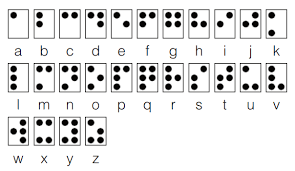
\includegraphics[width=1\textwidth]{Imagenes/Fuentes/SAAC/braille.png}
			\caption{Representaci�n del abecedario en el Sistema Braille}
			\label {fig: imgBraille}
		\end{figure}
		
		\item \textit{\textbf{Pictogramas:}} sistema que utiliza dibujos simples o s�mbolos para comunicarse de forma sencilla. Los s�mbolos son dise�ados con el fin de representar las palabras y conceptos de uso m�s com�n. Existen diversos sistemas pictogr�ficos, como por ejemplo MIC o ARASAAC, cuyos pictogramas son los m�s utilizados en Espa�a. En la Figura~\ref {fig: imgPictografico} se muestra la representaci�n de varios elementos comunes mediante pictogramas. 
		
		\begin{figure}[]
			\centering
			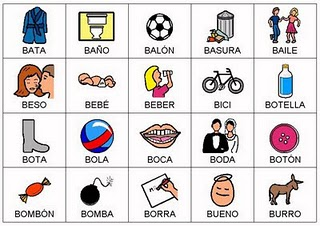
\includegraphics[width=0.9\textwidth]{Imagenes/Fuentes/SAAC/pictogramas.jpg}
			\caption{Representaci�n de distintas palabras con pictogramas}
			\label {fig: imgPictografico}
		\end{figure}
		
	\end{itemize}
\end{itemize}


%-------------------------------------------------------------------
\section{La Lengua de Signos}
%-------------------------------------------------------------------
\label{cap2:sec:La Lengua de Signos}

La Lengua de Signos (LS) \citep*{bkApuntesLing} es una lengua natural gestual que sirve para ayudar a integrarse a las personas con discapacidad auditiva o dificultad en el habla, y a personas que se quieran comunicar con ellas. La Lengua de Signos es considerada como SAAC gestual sin ayuda, es decir, no necesita apoyo de ning�n sistema de informaci�n (im�genes, pictogramas).\\ 

Esta lengua es rica y compleja gramaticalmente, es decir, no es una simple representaci�n literal de la lengua oral. Adem�s, es muy expresiva, ya que permite expresar sentimientos y emociones a la hora de comunicarse mediante el �nfasis en los gestos y expresiones faciales.\\

El desarrollo de esta lengua necesita de unas capacidades tanto cognitivas como motrices, as� como de un entrenamiento espec�fico. Este sistema puede tener una doble finalidad:

\begin{itemize}
	\item \textbf{Como elemento de comunicaci�n:} Para hacer posible la comunicaci�n de manera alternativa al habla o paliar las limitaciones que provoca la p�rdida auditiva y as� mejorar la integraci�n social de las personas que sufren esta discapacidad.
	
	
	
	\item \textbf{Como elemento de desarrollo intelectual:} la audici�n es el �rgano que m�s influye en la educaci�n, ya que es v�a de adquisici�n del lenguaje. El uso de estos sistemas es determinante en el desarrollo intelectual de las personas, sobre todo cuando el lenguaje verbal no est� adquirido.
	
\end{itemize}


La LS no es una lengua universal, es decir, no existe una Lengua de Signos com�n para todo el mundo ni para todos los idiomas. Cada pa�s puede contar con una o varias LS oficiales y no son �nicas para cada lengua. Esto quiere decir que dos pa�ses que comparten lengua oral oficial (como Espa�a y Argentina), tienen Lenguas de Signos totalmente diferentes. Incluso puede ocurrir que una misma LS presente diferencias dependiendo de en qu� regi�n del pa�s se utilice.\\

En Espa�a hay alrededor de 1.064.000 personas mayores de seis a�os con alg�n grado de discapacidad auditiva, de las cuales s�lo el 1,25\% (13.300 personas) utilizan la Lengua de Signos para comunicarse, seg�n los �ltimos datos aportados por el Instituto Nacional de Estad�stica (INE)\footnote{\url{https://www.ine.es/}}. Esto se debe  a que la mayor�a de las personas con esta discapacidad son capaces de comunicarse a trav�s del lenguaje oral, ya que su grado de discapacidad se lo permite y les ayuda a integrarse con el entorno debido a que no es com�n saber Lengua de Signos si no sufres de dicha discapacidad, siendo �nicamente alrededor de 400.000 las personas que saben comunicarse mediante dicha lengua en nuestro pa�s. Desde el a�o 2007 Espa�a cuenta con dos LS oficiales: la Lengua de Signos Espa�ola (LSE) y la Lengua de Signos Catalana (LSC), siendo la LSE la m�s utilizada en nuestro pa�s.\\


La LSE es una lengua normativizada, es decir, consta de unas reglas que marcan el correcto uso de la misma.

%-------------------------------------------------------------------
\subsection{Reglas de la Lengua de Signos Espa�ola}
%-------------------------------------------------------------------
A continuaci�n, se explica el conocimiento b�sico de estas normas en lo referente a la gram�tica, fonolog�a, sintaxis y morfolog�a.

%-------------------------------------------------------------------
\subsubsection{Fonolog�a de la Lengua de Signos Espa�ola}
%-------------------------------------------------------------------

La fonolog�a  \citep*{bkApuntesLing}, en lo relativo a la LSE,  se refiere al estudio de la estructura y organizaci�n interna de los signos.\\

Los signos de la LSE est�n formados por siete elementos esenciales:

\begin{itemize}
	\item \textbf{Forma o configuraci�n de la mano o manos} que intervienen en el signo. Es importante remarcar que no se utilizan los t�rminos ``mano izquierda'' y ``mano derecha'', ya que dependiendo de la persona, la mano dominante puede ser una u otra. Por eso se utilizan los t�rminos ``mano dominante'' y ``mano no dominante'' para se�alar con qu� mano o manos signar. Para indicar qu� mano es la dominante basta con levantarla y rotarla (tal y como se muestra en la Figura~\ref {fig: imgLSEConfig})
	
	\begin{figure}[]
		\centering
		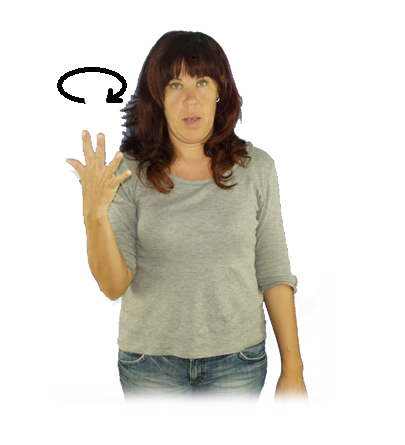
\includegraphics[width=0.5\textwidth]{Imagenes/Fuentes/SAAC/LSEConfig.png}
		\caption{Representaci�n de la configuraci�n de la mano en Lengua de Signos }
		\label {fig: imgLSEConfig}
	\end{figure}
	
	\item \textbf{Orientaci�n} de la mano o manos al signar respecto al cuerpo del individuo. Por ejemplo, gestos como \textit{``ayudar''}, el cual podemos observar en la Figura~\ref {fig: imgLSEAyudar}, van acompa�ados de direcci�n para indicar a qu� persona se refiere el emisor. En la Figura~\ref {fig: imgLSEOrient} se muestran las distintas direcciones que pueden acompa�ar a los gestos. 
	
	\begin{figure}[]
		\centering
		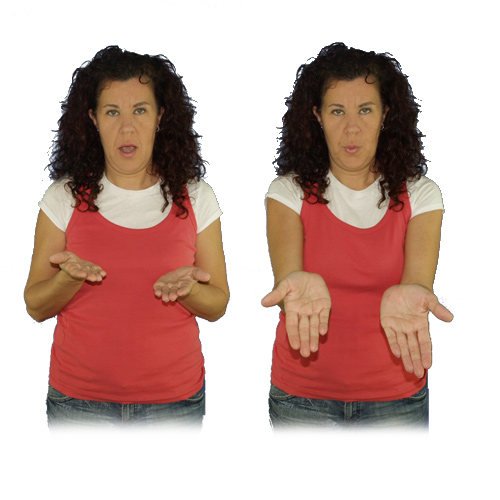
\includegraphics[width=0.45\textwidth]{Imagenes/Fuentes/SAAC/LSEAyudar.jpg}
		\caption{Signo \textit{``ayudar''} en LSE del banco de im�genes ARASAAC}
		\label {fig: imgLSEAyudar}
	\end{figure}
	
	\begin{figure}[]
		\centering
		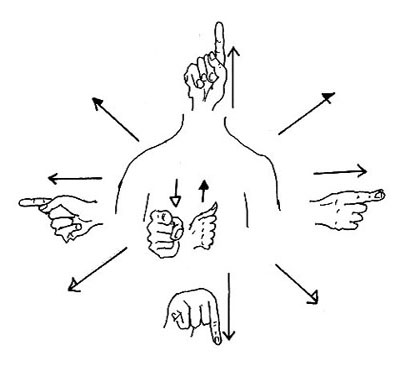
\includegraphics[width=0.5\textwidth]{Imagenes/Fuentes/SAAC/LSEOrient.jpg}
		\caption{Representaci�n de la orientaci�n de las manos en Lengua de Signos }
		\label {fig: imgLSEOrient}
	\end{figure}
	
	
	\item \textbf{Lugar de articulaci�n} del signo, es decir, el espacio en el que se realiza el movimiento. Puede ser ante el pecho, el hombro, la frente o los labios, entre otros. Por ejemplo, en la Figura~\ref {fig: imgLSEVisera}, el gesto referente a la palabra ``visera'' se realiza ante la frente.
	\item \textbf{Plano} en el que se realiza el signo, es decir, la distancia de realizaci�n del signo con respecto al cuerpo del individuo. Sirve para indicar el tiempo verbal de los gestos. Los gestos signados m�s cerca del cuerpo indican pasado y lo m�s alejados futuro.
	\item \textbf{Punto de contacto} de la mano dominante con el cuerpo del individuo al realizar el signo. Por ejemplo, al signar \textit{``oir''} el punto de contacto ser�a la oreja, tal y como se muestra en la Figura~\ref {fig: imgLSEPntContc}.
	
	\begin{figure}[]
		\centering
		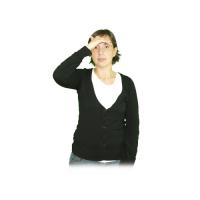
\includegraphics[width=0.5\textwidth]{Imagenes/Fuentes/SAAC/LSEVisera.jpg}
		\caption{Signo \textit{``visera''} en LSE del banco de im�genes ARASAAC }
		\label {fig: imgLSEVisera}
	\end{figure}
	
	\begin{figure}[]
		\centering
		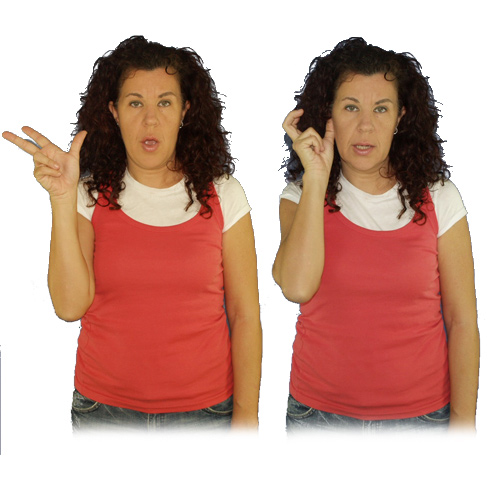
\includegraphics[width=0.5\textwidth]{Imagenes/Fuentes/SAAC/LSEPntContc.jpg}
		\caption{Signo \textit{``oir''} en LSE del banco de im�genes ARASAAC }
		\label {fig: imgLSEPntContc}
	\end{figure}
	
	
	\item \textbf{Movimiento} de las manos al realizar un signo. Puede ser giratorio, vaiv�n o quebrado, entre otros. Podemos observar en que consisten algunos de estos movimientos en la Figura~\ref {fig: imgLSEMovimientos}
	\item \textbf{Componente no manual} del signo, que puede ser desde expresiones faciales hasta movimientos corporales del individuo. Por ejemplo, en la Figura~\ref {fig: imgLSEMucho}, la int�rprete quiere expresar una cantidad abundante, acompa�ando al signo de una expresi�n facial que enfatiza una gran cantidad.
	
	\begin{figure}[]
		\centering
		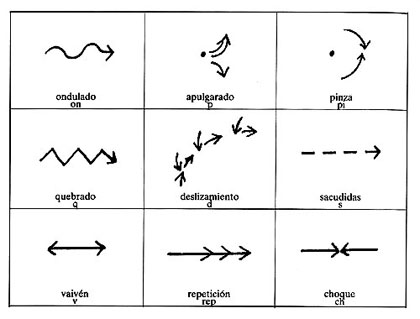
\includegraphics[width=1\textwidth]{Imagenes/Fuentes/SAAC/LSEMovimientos.jpg}
		\caption{Ejemplos de tipos de movimientos realizados al signar en LSE }
		\label {fig: imgLSEMovimientos}
	\end{figure}
	
	\begin{figure}[]
		\centering
		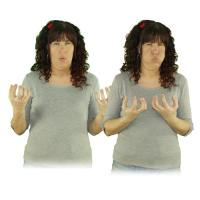
\includegraphics[width=0.5\textwidth]{Imagenes/Fuentes/SAAC/LSEMucho.jpg}
		\caption{Signo \textit{``mucho''} en LSE del banco de im�genes ARASAAC }
		\label {fig: imgLSEMucho}
	\end{figure}
\end{itemize}


%-------------------------------------------------------------------
\subsubsection{Sintaxis de la Lengua de Signos Espa�ola}
%-------------------------------------------------------------------

Las oraciones en la LSE no se estructuran igual que en castellano. La LSE es una lengua anal�tica, es decir, la estructura de las oraciones es muy simple, tendiendo a simplificar las frases para comunicar la informaci�n de la manera m�s concisa posible, al igual que lenguas como japon�s o alem�n.\\

La estructura b�sica de las oraciones se compone de sujeto-objeto-verbo, aunque existen excepciones. Por ejemplo, la oraci�n \textit{``�l come patatas''} en LSE se traducir�a como \textit{``�l patatas comer''}. Seg�n se van incorporando elementos a las oraciones, la estructura se va volviendo m�s compleja siguiendo un orden temporal, es decir, las acciones se nombran en el orden en el que suceden. Por ejemplo, la oraci�n \textit{``Despu�s de comer me fui a dormir''}, se traducir�a a LSE como \textit{``Yo comer fin dormir ir''}, indicando que primero se realiz� la acci�n de comer y despu�s la acci�n de irse a dormir.


%-------------------------------------------------------------------
\subsubsection{Morfolog�a de la Lengua de Signos Espa�ola}
%-------------------------------------------------------------------

En la lengua oral, los morfemas de g�nero sirven principalmente para marcar la concordancia entre el sustantivo y el adjetivo. En la LSE esto no existe, ya que tanto los adjetivos como los sustantivos son palabras invariables y adem�s, no existen los art�culos. Los elementos inanimados no tienen g�nero en la LSE, por lo que no es necesario signarlos, mientras que los elementos animados s� que precisan de distinci�n. En caso de que se quiera hacer �nfasis en el g�nero de alguna palabra, al terminar de signar la palabra en cuesti�n se a�aden los signos de  \textit{``hombre''} (Figura~\ref {fig: imgLSEHombre}) o de  \textit{``mujer''} (Figura~\ref {fig: imgLSEMujer}).\\


\begin{figure}[]
	\centering
	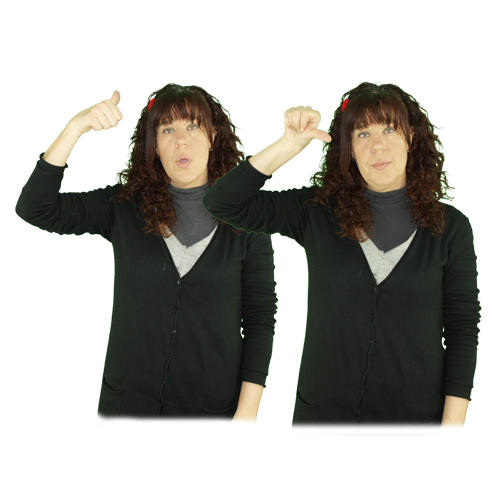
\includegraphics[width=0.45\textwidth]{Imagenes/Fuentes/SAAC/LSEHombre.jpg}
	\caption{Signo \textit{``hombre''} del banco de im�genes ARASAAC }
	\label {fig: imgLSEHombre}
\end{figure}

\begin{figure}[]
	\centering
	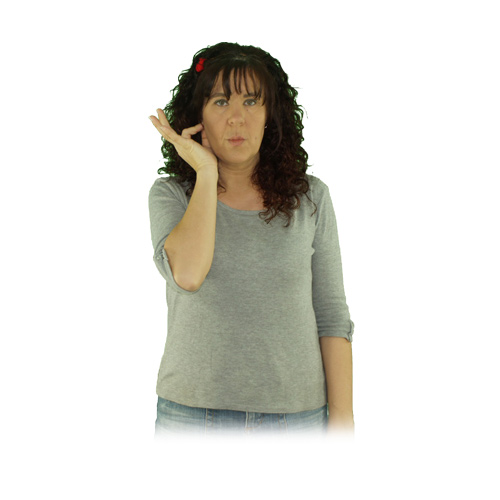
\includegraphics[width=0.4\textwidth]{Imagenes/Fuentes/SAAC/LSEMujer.jpg}
	\caption{Signo \textit{``mujer''} del banco de im�genes ARASAAC }
	\label {fig: imgLSEMujer}
\end{figure}

En las Figuras~\ref {fig: imgLSEAbuelo} y~\ref {fig: imgLSEAbuela} podemos observar c�mo se a�aden los signos \textit{``hombre''} y \textit{``mujer''} para marcar el g�nero de las palabras \textit{``abuela''} y \textit{``abuelo''}.\\

\begin{figure}[]
	\centering
	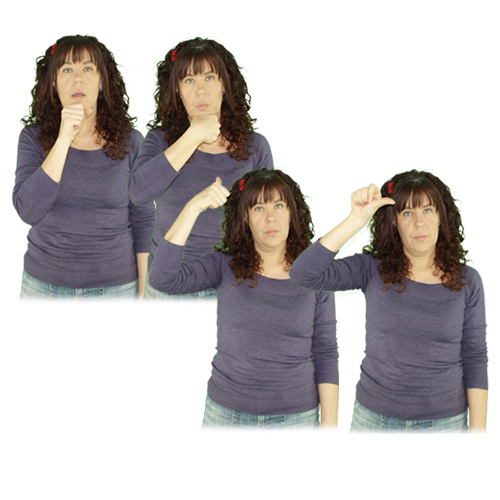
\includegraphics[width=0.45\textwidth]{Imagenes/Fuentes/SAAC/LSEAbuelo.jpg}
	\caption{Signo \textit{``abuelo''} del banco de im�genes ARASAAC }
	\label {fig: imgLSEAbuelo}
\end{figure}

\begin{figure}[]
	\centering
	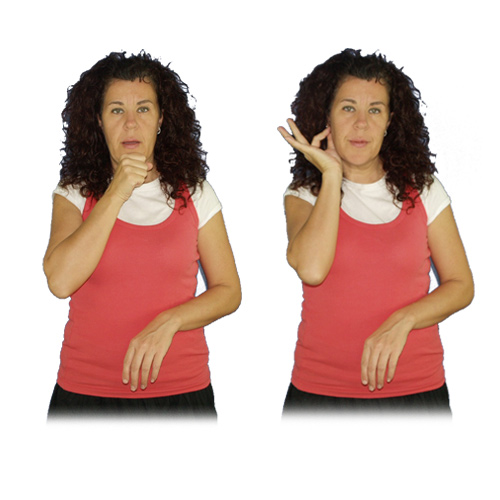
\includegraphics[width=0.4\textwidth]{Imagenes/Fuentes/SAAC/LSEAbuela.jpg}
	\caption{Signo \textit{``abuela''} del banco de im�genes ARASAAC }
	\label {fig: imgLSEAbuela}
\end{figure}


Existen algunas excepciones, como el caso de los signos para \textit{``ni�o''} y \textit{``ni�a''}, los cuales tienen su propio signo para definir el g�nero de la palabra. Podemos verlos en la Figura~\ref {fig: imgLSENi�o} y en la Figura~\ref {fig: imgLSENi�a} respectivamente.\\


\begin{figure}[]
	\centering
	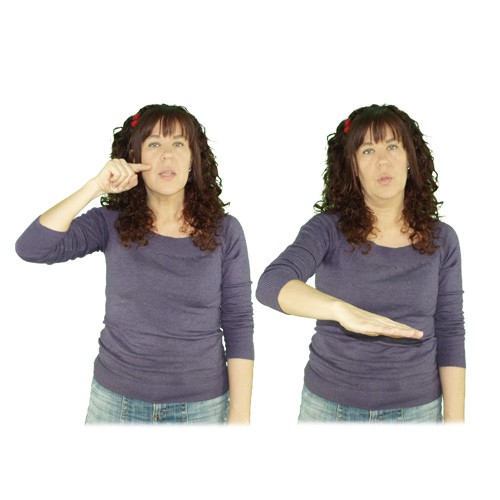
\includegraphics[width=0.45\textwidth]{Imagenes/Fuentes/SAAC/LSENino.jpg}
	\caption{Signo \textit{``ni�o''} del banco de im�genes ARASAAC }
	\label {fig: imgLSENi�o}
\end{figure}

\begin{figure}[]
	\centering
	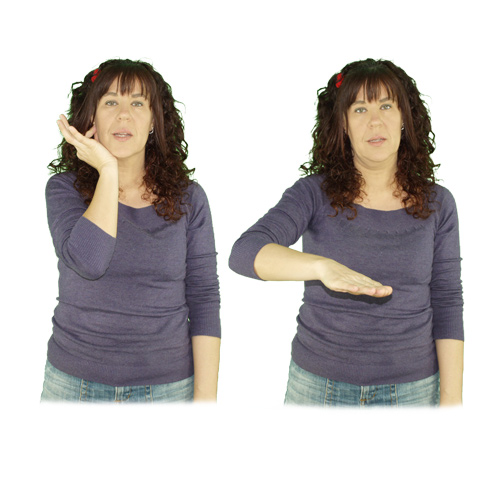
\includegraphics[width=0.45\textwidth]{Imagenes/Fuentes/SAAC/LSENina.jpg}
	\caption{Signo \textit{``ni�a''} del banco de im�genes ARASAAC }
	\label {fig: imgLSENi�a}
\end{figure}

Por otra parte, los morfemas de n�mero en la LSE sirven �nicamente para expresar cantidad. Existen varias formas de expresar cantidad seg�n la categor�a gramatical de la palabra a la que acompa�en:


\begin{itemize}
	
	\item \textbf{Sustantivos: }
	\begin{itemize}
		\item Si no queremos enfatizar el n�mero o queremos expresar solo una unidad, se signa la palabra sin a�adir nada a ella. Por ejemplo, la frase \textit{``La puerta de la universidad es de color gris''} en LSE ser�a \textit{``Universidad puerta color gris''}.\\
		
		\item Se pueden a�adir palabras que expresen cantidad, como cuantificadores definidos, por ejemplo \textit{``uno''}, cuyo signo podemos observar en la Figura~\ref {fig: imgLSEUno}, o cuantificadores indefinidos, por ejemplo \textit{``muchos''}, cuyo signo podemos observar en la Figura~\ref {fig: imgLSEMuchos}.\\
		
		\item Se puede enfatizar la cantidad de un sustantivo mediante la expresi�n facial de la cual se puede distinguir si es mucha o poca la cantidad a la que se quiere referir el emisor. Por ejemplo, en la Figura~\ref {fig: imgLSEMuchos} aparece una int�rprete realizando el signo \textit{``muchos''}. En ella podemos observar el gesto facial indicando una gran cantidad. Esta gesticulaci�n puede sustituir al propio signo \textit{``muchos''} en una oraci�n si se realiza mientras se signa la oraci�n.
		
	\end{itemize}
	
	
	\begin{figure}[]
		\centering
		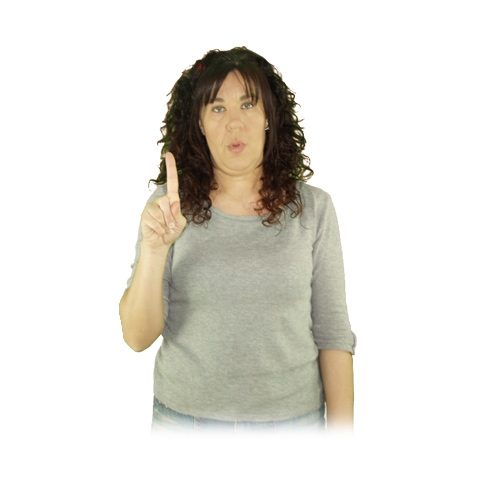
\includegraphics[width=0.45\textwidth]{Imagenes/Fuentes/SAAC/LSEUno.jpg}
		\caption{Signo \textit{``uno''} del banco de im�genes ARASAAC }
		\label {fig: imgLSEUno}
	\end{figure}
	
	\begin{figure}[]
		\centering
		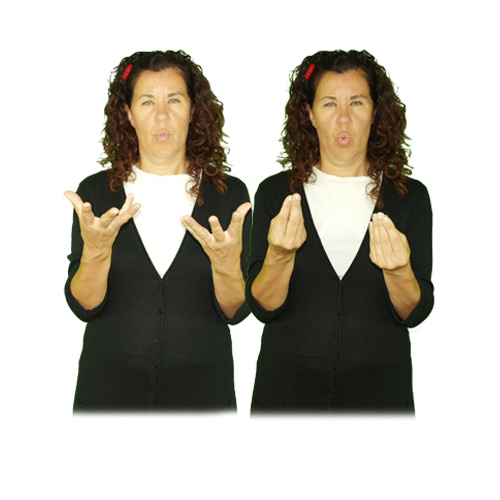
\includegraphics[width=0.45\textwidth]{Imagenes/Fuentes/SAAC/LSEMuchos.jpg}
		\caption{Signo \textit{``muchos''} del banco de im�genes ARASAAC }
		\label {fig: imgLSEMuchos}
	\end{figure}
	
	
	\item \textbf{Adjetivos:} no var�an en cuanto a n�mero.
	\item \textbf{Verbos:} el plural se realiza principalmente mediante la repetici�n del verbo y recae sobre el objeto. Por ejemplo, en la oraci�n \textit{``Yo viajo a muchos sitios''} se repetir�a el verbo viajar: \textit{``Yo viajar viajar sitio''}. \\
	
\end{itemize}

%-------------------------------------------------------------------
\subsubsection{Verbos de la Lengua de Signos Espa�ola}
%-------------------------------------------------------------------
El verbo en la LSE \citep*{tchVerbos} presenta unos rasgos gramaticales propios que es necesario tener en cuenta. Se distinguen tres clases b�sicas de verbos en LSE:

\begin{itemize}
	\item \textbf{Verbos planos:} Los verbos planos son aquellos cuyo signo no se modifica para marcar informaci�n complementaria, como por ejemplo el g�nero, el n�mero o a qui�n va dirigida la acci�n. Para a�adir este tipo de informaci�n se a�aden palabras independientes, como cuantificadores (uno, dos, etc), pronombres personales (yo, �l, etc). Por ejemplo, \textit{Querer, Comer, Pensar, Conducir, etc.} Podemos observar en la Figura~\ref {fig: imgLSEQuerer} como el signo de la palabra \textit{``Querer''} no aporta ning�n tipo de informaci�n adicional por s� mismo. 
	
	\item \textbf{Verbos de concordancia:} Los verbos de concordancia son aquellos que en la realizaci�n del propio signo se a�ade informaci�n adicional, como por ejemplo, a qui�n va dirigida la acci�n mediante la articulaci�n del signo. Esto podemos observarlo en la Figura~\ref {fig: imgLSEAyudar}, que muestra el signo de la palabra \textit{``ayudar''}, el cual termina se�alando en el espacio a la persona a la que se est� ayudando. Algunos ejemplos de verbos de concordacia son: \textit{Avisar, Ayudar, Contar, Cuidar, Responder, etc.} 
	
	
	\item \textbf{Verbos espaciales:} Los verbos espaciales son aquellos que no necesitan un signo espec�fico para expresar su significado, ya que indican la situaci�n en el espacio de algo o alguien a trav�s de la direcci�n y la velocidad con la que se realiza el signo. Al igual que en los verbos planos, se puede a�adir informaci�n adicional como g�nero o n�mero a trav�s de palabras independientes, como cuantificadores. Por ejemplo, \textit{``Hay un rat�n ah�''} se traduce como \textit{``Rat�n (Se�alando el sitio)''}. Esto podemos observarlo en la Figura~\ref {fig: imgLSESe�alar}, en la que se muestra el signo de la palabra \textit{``se�alar''}. 
	
	\begin{figure}[]
		\centering
		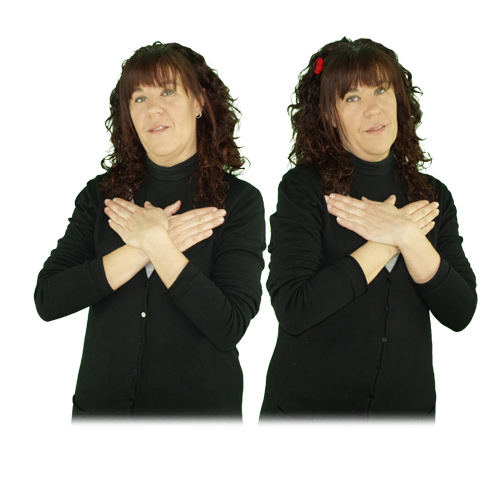
\includegraphics[width=0.45\textwidth]{Imagenes/Fuentes/SAAC/LSEQuerer.jpg}
		\caption{Signo \textit{``querer''} en LSE del banco de im�genes ARASAAC}
		\label {fig: imgLSEQuerer}
	\end{figure}
	
	
	
	\begin{figure}[]
		\centering
		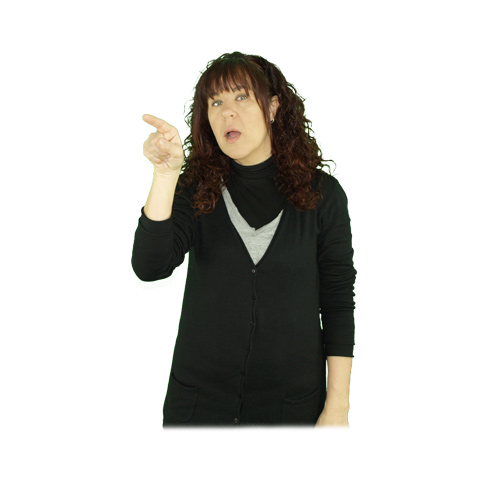
\includegraphics[width=0.45\textwidth]{Imagenes/Fuentes/SAAC/LSESenalar.jpg}
		\caption{Signo \textit{``se�alar''} en LSE del banco de im�genes ARASAAC}
		\label {fig: imgLSESe�alar}
	\end{figure}
	
\end{itemize} 


%-------------------------------------------------------------------
\subsection{Bancos de videos e im�genes LSE}
%-------------------------------------------------------------------

%-------------------------------------------------------------------
\subsubsection{ARASAAC}
%-------------------------------------------------------------------

El Portal Aragon�s de la Comunicaci�n Aumentativa y Alternativa (ARASAAC)\footnote {\url{http://www.arasaac.org/}}, es un proyecto desarrollado en el a�o 2007 por el gobierno de Arag�n. Tiene como objetivo la creaci�n de un sistema pictogr�fico de comunicaci�n y un conjunto de herramientas de libre distribuci�n. Estos recursos facilitan la accesibilidad de car�cter comunicativo y cognitivo en diversos �mbitos de la vida a todas las personas que lo puedan requerir. ARASAAC proporciona un cat�logo con m�s de 8.000 pictogramas en color, en blanco y negro, fotograf�as, as� como un banco de v�deos e im�genes a color de signos de la Lengua de Signos Espa�ola. En la Figura~\ref {fig: imgLSEHola} se muestra el signo \textit{``hola''} en LSE del banco de im�genes de LSE de ARASAAC. Este contenido est� disponible como contenido descargable con licencia Creative Commons, es decir, se puede usar libremente sin �nimo de lucro. \\

ARASAAC ofrece una API\footnote {\url{https://beta.arasaac.org/developers/api}} a trav�s de la cual se pueden obtener sus pictogramas y los materiales generados con sus pictogramas a trav�s de llamadas a los m�todos de dicha API. Para obtener los recursos correspondientes a la LSE es necesario descargarlos a trav�s del apartado de descargas de su p�gina web\footnote {\url{http://www.arasaac.org/descargas.php}}.


\begin{figure}[]
	\centering
	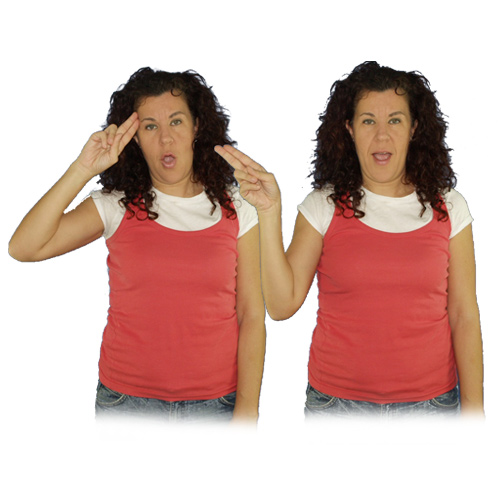
\includegraphics[width=0.45\textwidth]{Imagenes/Fuentes/SAAC/LSEHola.jpg}
	\caption{Signo \textit{``hola''} en LSE del banco de im�genes ARASAAC}
	\label {fig: imgLSEHola}
\end{figure}




%-------------------------------------------------------------------
\subsubsection{Banco de im�genes Fundacion CNSE}
%-------------------------------------------------------------------
La Confederaci�n Estatal de Personas Sordas (CNSE)\footnote{\url{http://www.fundacioncnse.org/}}  es una organizaci�n que  atiende los intereses de las personas sordas y sus familias en Espa�a. Es la primera entidad asociativa de la  discapacidad de nuestro pa�s, y desde su creaci�n se ha ocupado de incentivar el desarrollo y la participaci�n social de dicho colectivo. En ella se integran 17 federaciones de personas sordas, una por cada comunidad aut�noma, que, a su vez, mantienen afiliadas a m�s de 120 asociaciones provinciales y locales de todo el Estado. No obstante, la CNSE atiende cualquier necesidad relacionada con el colectivo de personas sordas, est�n o no afiliadas a su movimiento asociativo.\\

En 1998, la CNSE constituye la Fundaci�n CNSE para la Supresi�n de las Barreras de Comunicaci�n. Se trata de una organizaci�n estatal sin �nimo de lucro, desde la que se impulsa la investigaci�n y el estudio de la Lengua de Signos Espa�ola y se trabaja por mejorar la accesibilidad de las personas sordas en todos los �mbitos y se promueve el desarrollo de proyectos que mejoren la calidad de vida de las personas sordas y de sus familias.\\

Esta fundaci�n cuenta con un banco de im�genes\footnote{\url{http://www.fundacioncnse.org/educa/bancolse/}} (ver Figura~\ref {fig: imgFundCNSE}) y signos de la LSE, accesible a trav�s de su p�gina web. En esta p�gina no existe la opci�n de descargar todas las im�genes de una vez, sino que es necesario hacerlo manualmente una a una, y no cuenta con un banco de videos de signos.\\


\begin{figure}[]
	\centering
	\includegraphics[width=1\textwidth]{Imagenes/Fuentes/Apps/fundCNSE.png}
	\caption{Recursos LSE de la Fundaci�n CNSE}
	\label {fig: imgFundCNSE}
\end{figure}

%-------------------------------------------------------------------
\subsubsection{SpreadTheSign}
%-------------------------------------------------------------------
SpreadTheSign\footnote{\url{https://www.spreadthesign.com/es.es/search/}} es un diccionario online administrado por el Centro Europeo de Lenguas de Signos, que cuenta con m�s de 400.000 signos en v�deo (ver Figura~\ref {fig: imgSpreadTheSign}) de diferentes Lenguas de Signos, como la espa�ola, estadounidense o alemana, entre muchas otras, as� como de un alfabeto dactilol�gico para cada una de ellas y frases previamente almacenadas. Es una herramienta de autoaprendizaje gratuita, accesible a trav�s de su p�gina web y desde su aplicaci�n para Android\footnote{\url{https://play.google.com/store/apps/details?id=com.spreadthesign.androidapp_paid&hl=es}} e IOS\footnote{\url{https://apps.apple.com/ni/app/spreadthesign/id438811366}}, aunque ninguna de estas aplicaciones permite la descarga de contenido. 


\begin{figure}[]
	\centering
	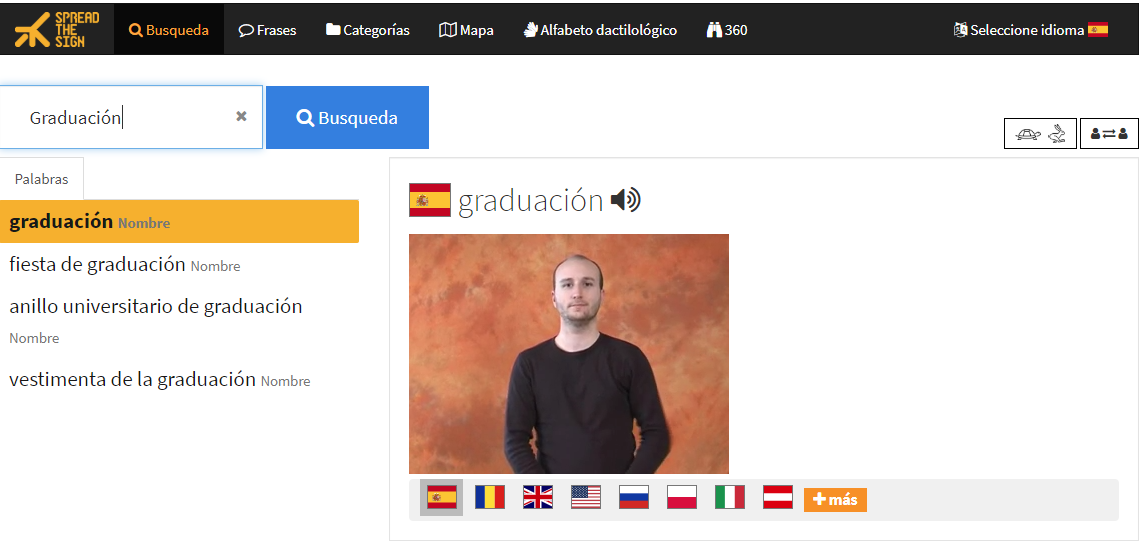
\includegraphics[width=1\textwidth]{Imagenes/Fuentes/Apps/SpreadTheSign_1.png}
	\caption{Imagen de la p�gina web SpreadTheSign}
	\label {fig: imgSpreadTheSign}
\end{figure}


%-------------------------------------------------------------------
\section{Aplicaciones de Traducci�n de Texto a LSE}
%-------------------------------------------------------------------
La variedad de recursos y aplicaciones orientadas a la integraci�n social de las personas con discapacidad auditiva ha ido aumentado con el paso del tiempo. En esta secci�n se presentan aplicaciones con un objetivo similar al de nuestro TFG cuyo prop�sito es ayudar en la integraci�n de las personas que sufren de discapacidad auditiva.


%-------------------------------------------------------------------
\subsection{Text2Sign}
\label{Text2Sign}
%-------------------------------------------------------------------
Text2Sign\footnote{\url{http://text2sign.es/}} es una aplicaci�n tanto web como m�vil gratuita que permite enviar un texto en formato PDF, imagen o Word a un equipo de int�rpretes que se encarga de traducirlo a la LSE. Una vez realizada la traducci�n se puede descargar a trav�s de la plataforma entre un periodo de 24 y 72 horas dependiendo de la longitud del texto ya que no es un servicio instant�neo y est� limitado a una o dos p�ginas.


%-------------------------------------------------------------------
\subsection{TextoSign}
%-------------------------------------------------------------------

TextoSign\footnote{\url{http://textosign.es/}} es una herramienta software que funciona en p�ginas web, asistentes virtuales y dispositivos m�viles que traduce en tiempo real un texto a la Lengua de Signos Espa�ola mediante un int�rprete visual llamado Maya (Figura~\ref {fig: imgTextSign}). Se trata de herramienta de pago y es utilizada hoy en d�a por La Caixa, Adif, Inturjoven y otras entidades.

\begin{figure}[]
	\centering
	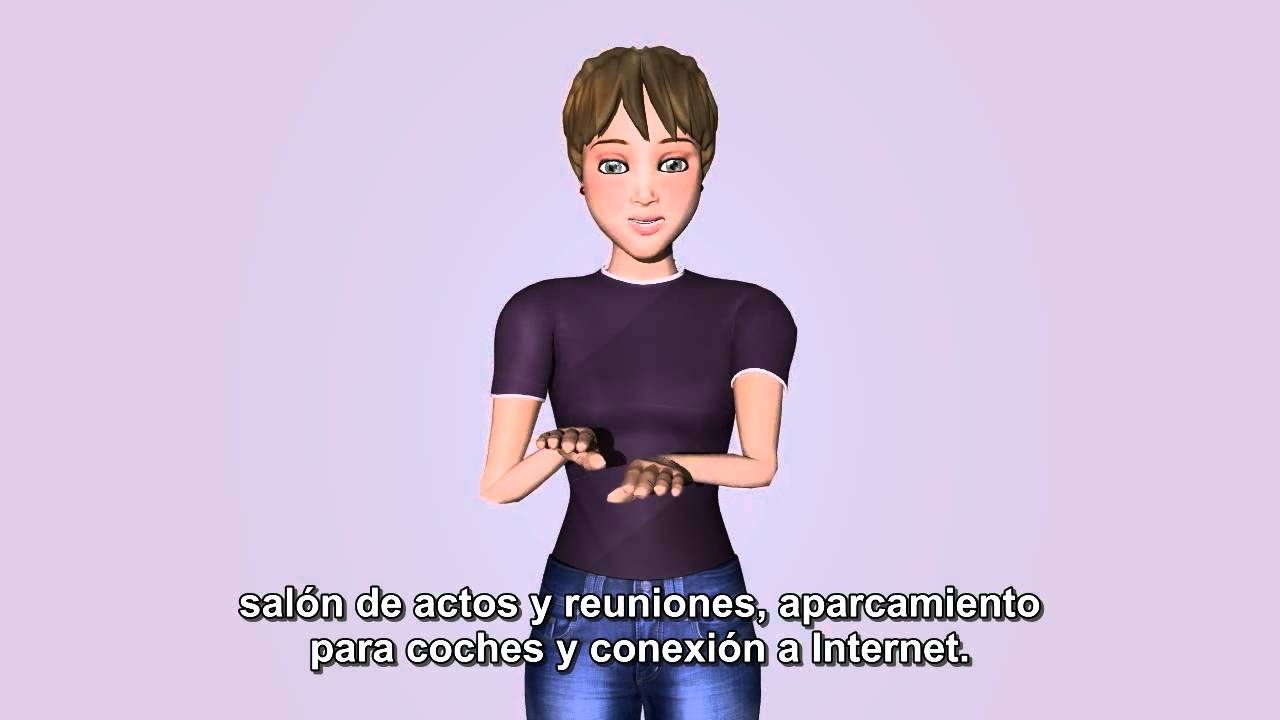
\includegraphics[width=0.8\textwidth]{Imagenes/Fuentes/Apps/textsign.jpg}
	\caption{Maya, avatar usado por TextoSign.}
	\label {fig: imgTextSign}
\end{figure}


%-------------------------------------------------------------------
\subsection{StorySign}
%-------------------------------------------------------------------
StorySign\footnote{\url{https://play.google.com/}} es una aplicaci�n para Android gratuita desarrollada por Huawei, que traduce en tiempo real  una selecci�n de cuentos infantiles a diferentes Lenguas de Signos como la espa�ola, italiana, francesa o inglesa. Para utilizarla es necesario abrir la aplicaci�n y sostener el m�vil encima del libro f�sico (especialmente dise�ado para esta aplicaci�n). Un avatar llamado Star interpreta el cuento en Lengua de Signos mientras la aplicaci�n resalta cada palabra que Star interpreta como podemos ver en la Figura~\ref {fig: imgStorySign}.

\begin{figure}[]
	\centering
	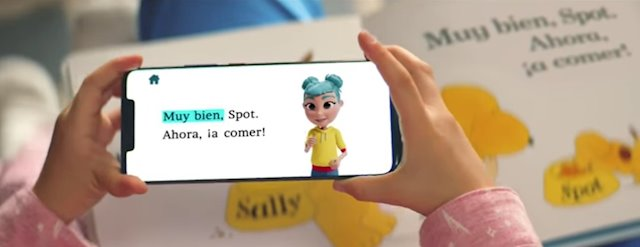
\includegraphics[width=1\textwidth]{Imagenes/Fuentes/Apps/storySign_1.jpg}
	\caption{Imagen de la aplicaci�n StorySign.}
	\label {fig: imgStorySign}
\end{figure}

%-------------------------------------------------------------------
\subsection{TeCuento}
%-------------------------------------------------------------------
TeCuento\footnote{\url{https://play.google.com/}}  es una aplicaci�n Android gratuita que contiene diversos cuentos que se reproducen en video con subt�tulos y LSE, como podemos apreciar en la Figura~\ref {fig: imgTeCuento}. No se traduce en el momento, son videos previamente grabados por personas f�sicas dando tambi�n la opci�n de poder escribir tu propio cuento y que lo traduzcan a LSE.



\begin{figure}[]
	\centering
	
\includegraphics[width=1\textwidth]{Imagenes/Fuentes/Apps/teCuento_1.png}
	\caption{Imagen de la aplicaci�n TeCuento.}
	\label {fig: imgTeCuento}
\end{figure}

%-------------------------------------------------------------------
\subsection{Conclusiones}
%-------------------------------------------------------------------


Como se ha podido comprobar existe un abanico amplio de aplicaciones que son capaces de traducir texto a LSE. Estas herramientas en su mayor�a cumplen el prop�sito de facilitar el uso de la Lengua de Signos a las personas que quieran comunicarse con ella. No obstante, presentan algunas limitaciones como licencias de pago, tiempo de respuesta lento o disponibilidad en un solo tipo de dispositivo.\\

Nuestro proyecto Text2LSE pretende solventar muchas de estas limitaciones proporcionando una aplicaci�n gratuita que sea accesible desde cualquier dispositivo, ya sea web o m�vil. El objetivo es ofrecer una traducci�n al instante de cualquier frase o palabra en castellano a LSE y la posibilidad de integrarse mediante servicios web en aplicaciones que requieran su uso.























%---------------------------------------------------------------------
%
%                          Cap�tulo 3
%
%---------------------------------------------------------------------

\chapter{Herramientas utilizadas}

\begin{FraseCelebre}
	\begin{Frase}
		"Controlar la complejidad es la esencia de la programaci�n". 
	\end{Frase}
	\begin{Fuente}
		Brian Kernigan
	\end{Fuente}
\end{FraseCelebre}


Introducci�n capitulo 3 COMPLETAR 
\\



%-------------------------------------------------------------------
\section{Python}
%-------------------------------------------------------------------
\label{cap3:sec:Python}

Python \citep*{tchDesarrolloWeb} es un lenguaje de programaci�n desarrollado a lo largo de la d�cada de los a�os 80 por Guido Vam Rossum. El objetivo del creador era desarrollar un lenguaje de programaci�n orientado a objetos de uso sencillo que sirviese para programar diversos tipos de tareas, no limitarlo a un solo tipo de uso. Sus principales caracter�sticas son:

\begin{itemize}
	
	\item \textbf{Din�mico:} Se puede utilizar para desarrollar desde simples scripts o p�ginas web hasta para servidores de gran potencia.
	
	\item \textbf{Interpretado:} El programador no necesita realizar el paso de compilar el c�digo, ya que Python se encarga de hacer esa compilaci�n por s� mismo de manera que el desarrollador  no tiene que realizar ese paso extra.
	
	\item \textbf{Multiplataforma:} Se puede utilizar en cualquier sistema inform�tico, siempre y cuando se haya instalado previamente un int�rprete compatible con �l.
	
	\item \textbf{Interactivo:} Python contiene un int�rprete por l�nea de comandos, a trav�s del cual se pueden introducir sentencias y ver en tiempo real el resultado de dicha sentencia.
	
	\item \textbf{Orientado a objetos:} el c�digo se estructura en elementos llamados clases, a trav�s de las cuales se crean los objetos con funcionalidades espec�ficas.
	
	\item \textbf{Funciones y librer�as:} python incluye una serie de funciones incluidas de base, como por ejemplo, la manipulaci�n de strings, n�meros, etc. A parte, existen multitud de librer�as que se pueden importar al desarrollar un programa para cubrir necesidades espec�ficas, como por ejemplo, el procesamiento del lenguaje natural.
	
	\item \textbf{Sintaxis clara:} La estructura del c�digo se basa en los m�rgenes de obligado cumplimiento, siendo as� muy visual. Esto hace que sea m�s sencillo distinguir las distintas partes del c�digo.
	
	\item \textbf{Licencia de c�digo abierto} \citep*{tchPython}: Licencia compatible con la Licencia p�blica general de GNU, la cual permite que el usuario final pueda tener acceso al c�digo, descargarlo, copiarlo y manipularlo.
	
\end{itemize}

Se ha decidido utilizar Python en este proyecto debido a la facilidad de uso y a la existencia de diversas librer�as de procesamiento de lenguaje natural, como Spacy y NLTK, las cuales se describen en los apartados previos \hyperref[cap2:sec:PLN:subsec:Spacy]{``Spacy''} y \hyperref[cap2:sec:PLN:subsec:NLTK]{``NLTK''} respectivamente.



%-------------------------------------------------------------------
\section{Flask}
%-------------------------------------------------------------------
\label{cap2:sec:Flask}
Flask es un ``micro'' Framework escrito en Python y concebido para facilitar el desarrollo de Aplicaciones Web y APIs.\\

La palabra micro hace referencia a que Flask �nicamente trae por defecto las herramientas necesarias para crear una aplicaci�n web b�sica, aunque si se necesitan a�adir nuevas funcionalidades hay un conjunto muy grande de extensiones (plugins) que se pueden instalar f�cilmente. Por ello, Flask es muy recomendable para el desarrollo de aplicaciones que no requieran muchas extensiones o que se necesiten implementar de una forma �gil y r�pida. Tambi�n es muy recomendable para implementar microservicios.\\

Algunas de las caracter�sticas de Flask por las que decidimos desarrollar nuestra API con este framework son las siguientes:\\

\newpage
\begin{itemize}
	
	\item Rapidez y facilidad en la instalaci�n y configuraci�n, a diferencia de otros frameworks como Django, que tiene una curva de aprendizaje mucho m�s baja.
	
	\item Es compatible con Python. Nuestra API est� implementada en dicho lenguaje.
	
	\item Incluye un servidor web de desarrollo. No se necesita una infraestructura con un servidor web para probar las aplicaciones, sino que de una manera sencilla se puede levantar un servidor web para ir viendo los resultados que se van obteniendo.
	
	\item Cuenta con depurador. Si tenemos alg�n error en el c�digo que se est� desarrollando, se puede depurar ese error y ver los valores de las variables.
	
	\item Flask es Open Source y est� amparado bajo una licencia BSD, que es la licencia utilizada para los sistemas operativos BSD (Berkeley Software Distribution), y tiene menos restricciones en comparaci�n con otras licencias como la GPL, estando muy cercana al dominio p�blico.
	
	\item Cuenta con una muy buena documentaci�n.
	
\end{itemize}


%-------------------------------------------------------------------
\section{Nginx}
%-------------------------------------------------------------------
\label{cap2:sec:Nginx}

Nginx \footnote{Web oficial de Nginx \url{https://www.nginx.com/}} es un servidor web de alto rendimiento, capaz de trabajar junto con diversas tecnolog�as de desarrollo y lenguajes. La asincron�a es una de sus caracter�sticas fundamentales, junto con su rapidez, debido a que es un servidor web ligero.
A d�a de hoy, adem�s de sus capacidades de servidor HTTP, NGINX tambi�n puede funcionar como un servidor proxy para correo electr�nico (IMAP, POP3 y SMTP) y un proxy inverso y equilibrador de carga para servidores (HTTP, TCP y UDP).\\

Las ventajas de NGINX y el porqu� de su uso:

\begin{itemize}
	
	\item Nginx es un software multiplataforma que se puede usar en la gran mayor�a de los sistemas operativos, tanto en sistemas basados en Unix como en Windows.
	
	\item Consume menos recursos que la mayor�a de servicios que hacen su misma funci�n ya que hace un uso de memoria de forma est�tica y se mantiene bastante estable independientemente del volumen de tr�fico.
	
	\item Proporciona un alto rendimiento sobre todo en casos de mucho tr�fico.
	
	\item Puede ser usado como Proxy inverso cacheando el contenido de nuestros sitios web.
	
	
\end{itemize}















%---------------------------------------------------------------------
%
%                          Cap�tulo 4
%
%---------------------------------------------------------------------

\chapter{Metodolog�as utilizadas}

\begin{FraseCelebre}
	\begin{Frase}
		"Juntarse es un comienzo. Seguir juntos es un progreso. Trabajar juntos es un �xito". 
	\end{Frase}
	\begin{Fuente}
		Henry Ford
	\end{Fuente}
\end{FraseCelebre}

En este cap�tulo se habla de la metodolog�a de trabajo seguida por el equipo de este TFG durante el desarrollo del mismo, junto con algunas de las herramientas utilizadas para organizar y estructurar las tareas a realizar por cada uno de los miembros y mantener el c�digo de la aplicaci�n accesible y con sus correspondientes copias de seguridad. COMPLETAR

%-------------------------------------------------------------------
\section{Metodolog�as �giles}
%-------------------------------------------------------------------
\label{cap4:sec:Metodologias Agiles}

Las metodolog�as �giles \citep*{tchMetAgiles} son aquellas que permiten adaptar la forma de trabajo a las condiciones particulares de cada proyecto, consiguiendo flexibilidad e inmediatez en la respuesta para amoldar el proyecto y su desarrollo a las circunstancias espec�ficas del entorno.\\


La aplicaci�n de metodolog�as �giles permite involucrar a nuestros tutores a lo largo de todo el proyecto. En cada etapa se informa de los logros y progresos del mismo, con la visi�n de involucrarles directamente para sumar su experiencia y conocimiento, y as� optimizar las caracter�sticas del resultado final, obteniendo en todo momento una visi�n completa de su estado. La continua interacci�n entre los alumnos y los tutores tiene como objetivo asegurar que el resultado final sea exactamente lo que se busca y necesita. Adem�s, es posible detectar de forma r�pida tanto errores como problemas que puedan aparecer a lo largo del proyecto, por lo que es posible dar respuesta a todos aquellos contratiempos que puedan darse desde el inicio. Todo esto es posible gracias a las constantes reuniones que se realizan tanto entre los integrantes del grupo como entre los alumnos y los tutores. Estas reuniones se explican con m�s en detalle en la secci�n 4.x.\\

Adem�s, el trabajo se realiza con mayor velocidad y eficiencia, ya que se trabaja a trav�s de entregas parciales del proyecto. De este  modo, es posible entregar en el menor intervalo de tiempo posible una versi�n mucho m�s funcional de la aplicaci�n y de la memoria. La herramienta elegida para gestionar el trabajo realizado ha sido el conocido controlador de versiones Git, del que se habla con detalle en la secci�n 4.x.\\


Desde el comienzo, una de las mayores ventajas de la utilizaci�n de metodolog�as �giles es la mejora de la implicaci�n de los integrantes del equipo. Estas metodolog�as permiten a todos los miembros conocer el estado del proyecto en cualquier momento, y facilita tanto el reparto de tareas como que los compromisos sean acordados y aceptados por todos. La herramienta utilizada para organizar todo el trabajo ha sido Trello, explicada en la secci�n 4.x.\\


Existen diversas modalidades de metodolog�as �giles, algunas de las m�s conocidas son Scrum o Programaci�n Extrema (XP). Concretamente, para el desarrollo de este proyecto se ha optado por la utilizaci�n de Kanban, que se explica en detalle en la secci�n 4.x.


%-------------------------------------------------------------------
\section{Kanban}
%-------------------------------------------------------------------
\label{cap4:sec:Kanban}

Kanban \citep*{tchKanban1} es una metodolog�a agile cuyo objetivo es gestionar de manera general c�mo se van completando las tareas a llevar a cabo. Kanban es una palabra japonesa que significa 'tarjetas visuales', donde Kan es 'visual', y Ban corresponde a 'tarjeta'.\\

Las principales ventajas de esta metodolog�a es que es muy f�cil de utilizar, actualizar y asumir por parte del equipo. Adem�s, destaca por ser una t�cnica de gesti�n de las tareas muy visual, que permite ver a golpe de vista el estado de los proyectos, as� como tambi�n pautar el desarrollo del trabajo de manera efectiva. La herramienta utilizada para gestionar las tareas a realizar por los miembros del equipo ha sido Trello, explicada con detalle en la secci�n 4.x.\\


En Kanban existen una serie de principios b�sicos \citep*{tchKanban2} que ayudan a obtener el m�ximo rendimiento del flujo de trabajo. Algunos de los que hemos aplicado en nuestro proyecto son los siguientes:\\

\begin{itemize}
	
		\item \textbf{Visualizar lo que hace el flujo de trabajo:} una visualizaci�n de todas las tareas contribuye a que todos los miembros del equipo nos mantengamos al corriente de nuestro trabajo. Todos los miembros del equipo somos capaces de trabajar en el mismo tablero y colaborar en tiempo real. Adem�s, el tablero digital Trello, a trav�s de su aplicaci�n m�vil, nos permiten acceder a nuestro flujo de trabajo desde cualquier sitio, compartir tareas con facilidad y comunicarnos entre nosotros.
		
		\item \textbf{Limitar la cantidad de Trabajo en Proceso:} establecer metas asequibles y limitar los trabajos en proceso para prevenir el exceso de cantidad de tareas, que ser�an muy dif�ciles de completar.
		
		\item \textbf{Lectura f�cil de indicadores visuales:} con Kanban es sencillo conocer lo que est� ocurriendo de un solo vistazo. Utilizamos tarjetas de colores para distinguir los tipos de trabajo, prioridades, o fechas l�mite. 

\end{itemize}



%-------------------------------------------------------------------
\section{Trello}
%-------------------------------------------------------------------
\label{cap4:sec:Trello}

A lo largo de todo el proyecto se ha utilizado la herramienta Trello\footnote {\url{https://trello.com/}} para el reparto claro y equitativo de tareas entre los componentes del equipo de trabajo. Trello consiste en un conjunto de tableros, a los cuales se les pueden a�adir una serie de tareas con diferentes estados. Esto podemos observarlo en la Figura~\ref {fig: imgTrello} , donde se muestra un ejemplo de tablero utilizado en el desarrollo del proyecto. Esta herramienta permite ver de manera sencilla el estado del proyecto, facilitando as� la organizaci�n de las tareas a realizar. En el desarrollo de ``Text2LSE'' se han utilizado tres tableros distintos:

\begin{itemize}
	
	\item \textbf{Investigaci�n:} Incluye las tareas relacionadas con toda la investigaci�n referente al proyecto, como por ejemplo LSE, Python, PLN, etc.
	
	\item \textbf{Desarrollo:} Este tablero contiene las distintas tareas de desarrollo de c�digo, tanto de la aplicaci�n web como de la API.
	
	\item \textbf{Memoria:} En este tablero se encuentran las distintas tareas relacionadas con el desarrollo y correcci�n de los apartados de la memoria.
	
\end{itemize}

Para una mayor organizaci�n, cada tablero se ha estructurado en tres estados:

\begin{itemize}
	
	\item \textbf{Lista de Tareas:} Lista de tareas asignadas a un miembro del equipo en concreto que todav�a est�n sin empezar.
	
	\item \textbf{En proceso:} Tareas que el propietario de la tarjeta tiene en proceso de desarrollo. 
	
	\item \textbf{Hecho:} Tareas completadas y subidas al repositorio de GitHub.
	
\end{itemize}

Cada miembro del equipo ha sido el encargado de actualizar en tiempo real el estado de las tarjetas que ten�a asignadas. De esta manera se ha conseguido tener una buena organizaci�n con respecto a las tareas a realizar.

\begin{figure}[]
	\centering
	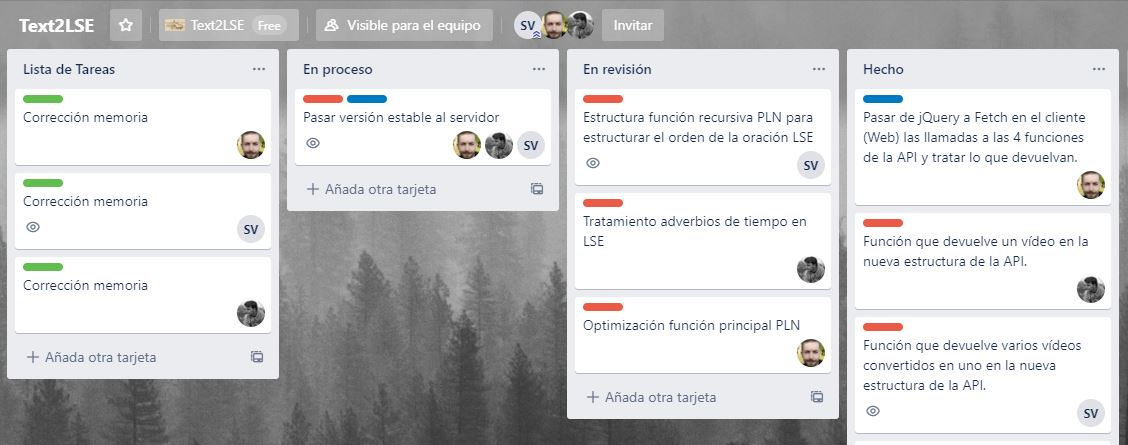
\includegraphics[width=1\textwidth]{Imagenes/Fuentes/Metodologias/trello.jpg}
	\caption{Tablero \textit{``Memoria''} utilizado en el proyecto.  }
	\label {fig: imgTrello}
\end{figure}
 


%-------------------------------------------------------------------
\section{Reuniones}
%-------------------------------------------------------------------
\label{cap4:sec:Reuniones}

Para una buena organizaci�n, desde el principio el equipo de trabajo se ha reunido una vez a la semana para asignar las diferentes tareas, comentar el trabajo realizado y poner en com�n todos los conocimientos adquiridos por cada uno. A lo largo de la semana tambi�n hab�a reuniones a trav�s de Skype\footnote {\url{https://www.skype.com/es/}} para comentar y resolver las posibles dudas que podr�an surgir durante el proceso. \\

El equipo tambi�n se ha mantenido en contacto v�a email con los tutores comentando el estado del proyecto. A esto se a�adieron reuniones mensuales con ellos para realizar correcciones de la memoria, revisar el progreso, resolver dudas y comentar las tareas necesarias para las siguientes fases.\\

De esta forma, los integrantes del equipo y los tutores han estado informados constantemente del progreso del trabajo, se ha podido hacer un reparto claro de tareas y se han podido establecer tiempos de entregas realistas y factibles.\\


%-------------------------------------------------------------------
\section{Control de versiones}
%-------------------------------------------------------------------
\label{cap4:sec:Control de versiones}
\subsection{GIT}

Para el desarrollo del proyecto se ha utilizado Git \footnote{Web oficial de Git \url{https://git-scm.com/}} que es un sistema de control de versiones distribuido que sirve para trabajar en equipo de una manera muy sencilla y optimizada. Git permite al usuario tener un control absoluto de su proyecto pudiendo ver todos los cambios realizados en nuestra aplicaci�n y nuestro c�digo por cada uno de los miembros o incluso volver a versiones anteriores del proyecto.

Sus principales herramientas son:

\begin{itemize}
	
	\item \textbf{Repository:} es un directorio donde se almacenan los archivos de tu proyecto. Puede estar ubicado en el almacenamiento de GitHub o en un repositorio local en tu computadora y tenerlos sincronizados.
	
	
	\item \textbf{Branch:} es una copia de tu repositorio cuyo desarrollo es independiente al repositorio central u otras ramas. Una vez realizados los cambios se puede combinar tu rama con otras ramas y con el repositorio central mediante un request.
	 
	
	\item \textbf{Commits:} son los cambios realizados en los archivos de tu repositorio local.

	\item \textbf{Pull:} acci�n que actualiza el repositorio local de tu ordenador con la �ltima versi�n del proyecto alojado en Github.
	
	\item \textbf{Push:} permite subir a Github los commits realizados en el repositorio local.	
	
\end{itemize}


\subsection{GITHUB}
GitHub \footnote{Web oficial de Github \url{https://help.github.com/}} es una plataforma que proporciona una interfaz que mediante las herramientas del control de versiones Git permite ver y llevar el registro de todos los cambios realizados en nuestro proyecto, organizarlos y resolver cualquier conflicto que pueda surgir. \\

Github tambi�n funciona como una red social para desarrolladores ya que permite a otros usuarios ver y colaborar en tus repositorios as� como resolver dudas que se tengan.






%---------------------------------------------------------------------
%
%                          Trabajo individual
%
%---------------------------------------------------------------------

\chapter{Trabajo individual}


%-------------------------------------------------------------------
\section{Sara Vegas Ca�as}
%-------------------------------------------------------------------
\label{capTrabajoIndividual:sec:Sara}

Lo primero de todo fue una investigaci�n profunda de la discapacidad auditiva y de la Lengua de Signos Espa�ola por parte de los tres integrantes de este proyecto, de esta manera todos nos concienciamos de las dificultades que tienen todas las personas sordas para comunicarse en su d�a a d�a. Realic� una investigaci�n de las herramientas que tienen estas personas a su disposici�n, tanto posibles traductores a LSE, como bancos de v�deos e im�genes. Encontr� una variedad de aplicaciones, las cuales prob� para poder ver hasta donde llegaban las soluciones actuales para el problema de comunicaci�n de las personas sordas. \\

Cuando llegamos a la conclusi�n del proyecto que quer�amos hacer, empezamos con la investigaci�n de las posibles tecnolog�as que podr�amos usar en el proyecto. Mi investigaci�n en este tema se centr� en servicios web, sobre todo de tipo REST, Python y en Procesamiento del Lenguaje Natural, probando diferentes librer�as, como Spacy y NLTK, para poder elegir la que m�s se ajustase a nuestras necesidades.\\

Una vez que termin� la primera parte de investigaci�n, nos reunimos para juntar todas nuestras conclusiones y comenzamos a desarrollar la primera parte de la memoria con los conocimientos adquiridos en la investigaci�n previa.\\

A continuaci�n, comenzamos a crear una primera base de la aplicaci�n. Lo primero fue realizar la preparaci�n del entorno local en Debian 10, utilizando Nginx para alojar la aplicaci�n web, y Flask para ejecutar la API, preparando el modo debug para el posterior proceso de desarrollo de c�digo. Construimos una web b�sica, en la cual pod�amos escribir un texto y enviarlo a la API a trav�s de JavaScript, mediante jQuery y Ajax, y una primera estructura de la API REST en Python. En este apartado me encargue junto con mi compa�ero Alejandro del desarrollo de una funcionalidad javascript capaz de lanzar una petici�n a la API con el texto y que esta nos devolviese un video mp4.\\

En la fase posterior, me encargu� de corregir mis apartados correspondientes de la memoria, y de desarrollar los nuevos apartados de Python y metodolog�as utilizadas como Trello y Reuniones. Tambi�n me encargu� de estructurar la funci�n de la API que devuelve un video con varios signos y de desarrollar las llamadas a las funciones que devuelven diferente tipo de informaci�n en Json. Respecto a PLN, en un principio me centr� en desarrollar un algoritmo que recorra un �rbol de dependencias desde el verbo a partir de una frase.\\


%-------------------------------------------------------------------
\section{Alejandro Torralbo Fuentes}
%-------------------------------------------------------------------


Al comienzo del proyecto, los tres integrantes del grupo realizamos una fase de investigaci�n, en la que adquirimos conocimientos sobre la discapacidad auditiva y la Lengua de Signos, y nos pusimos al d�a en los problemas a los que se enfrenta el colectivo de personas sordas, para poder orientar nuestro proyecto a solucionar dichos problemas. A continuaci�n, realizamos una b�squeda de recursos que pudi�ramos utilizar en el desarrollo de nuestra aplicaci�n, encontrando bancos de im�genes y v�deos de Lengua de Signos Espa�ola como la de ARASAAC, entre otras herramientas.\\

Una vez recopilada la informaci�n necesaria, comenzamos con la instalaci�n y preparaci�n del entorno de desarrollo local: una m�quina virtual con Debian 10, en la que instalamos un servidor para alojar el cliente con nginx, y una api desarrollada en python y ejecutada mediante flask. Me encargu� de configurar el entorno flask, activando el modo debug para poder empezar a depurar el c�digo de la API, e instal� la herramienta Postman para la realizaci�n de pruebas y el controlador de versiones Git, para trabajar en el c�digo de forma conjunta con el resto de compa�eros.\\

A partir de este punto, comenzamos con el desarrollo de la aplicaci�n. Me encargu� de desarrollar una web responsive con html, css y javascript, alojada en el servidor nginx. Junto con mi compa�era Sara, conseguimos implementar una funci�n en  Ajax, que realiza una petici�n POST a la API, enviando el texto introducido por el usuario y recibiendo un v�deo en formato .mp4 para mostrarlo en la web. Adem�s, me encargu� de que la API fuera capaz de juntar varios v�deos en funci�n del texto recibido, y prepararlo para enviarlo a la p�gina web. Posteriormente los tres integrantes decidimos estructurar la API y dividir esta funcionalidad en varias funciones diferentes, de modo que el usuario interesado en utilizar nuestra API cuente con varias opciones de llamada. Mis compa�eros Miguel y Sara se encargaron de dividir esta funci�n.\\

Por otro lado, decidimos cambiar las llamadas AJAX de la web  por llamadas Fetch, y yo me encargu� de programar estas llamadas con ayuda de mi compa�era Sara. \\

Junto con el trabajo t�cnico, tambi�n particip� en la redacci�n y correcci�n  de la memoria, en la que trabajamos los tres compa�eros conjuntamente. Me encargu� de la correcci�n del cap�tulo 1 y parte del cap�tulo 2. Adem�s, desarroll� el apartado de Flask del cap�tulo 3,  y metodolog�as agiles y kanban en el cap�tulo 4.\\

%\include{...}
%\include{...}
%\include{...}
%\include{...}

% Apéndices
%\appendix
%%---------------------------------------------------------------------
%
%                          Parte 3
%
%---------------------------------------------------------------------
%
% Parte3.tex
% Copyright 2009 Marco Antonio Gomez-Martin, Pedro Pablo Gomez-Martin
%
% This file belongs to the TeXiS manual, a LaTeX template for writting
% Thesis and other documents. The complete last TeXiS package can
% be obtained from http://gaia.fdi.ucm.es/projects/texis/
%
% Although the TeXiS template itself is distributed under the 
% conditions of the LaTeX Project Public License
% (http://www.latex-project.org/lppl.txt), the manual content
% uses the CC-BY-SA license that stays that you are free:
%
%    - to share & to copy, distribute and transmit the work
%    - to remix and to adapt the work
%
% under the following conditions:
%
%    - Attribution: you must attribute the work in the manner
%      specified by the author or licensor (but not in any way that
%      suggests that they endorse you or your use of the work).
%    - Share Alike: if you alter, transform, or build upon this
%      work, you may distribute the resulting work only under the
%      same, similar or a compatible license.
%
% The complete license is available in
% http://creativecommons.org/licenses/by-sa/3.0/legalcode
%
%---------------------------------------------------------------------

% Definici�n de la �ltima parte del manual, los ap�ndices

%\partTitle{Ap�ndices}

%\makepart

%%---------------------------------------------------------------------
%
%                          Ap�ndice 1
%
%---------------------------------------------------------------------

\chapter{As� se hizo...}
\label{ap1:AsiSeHizo}

\begin{FraseCelebre}
\begin{Frase}
...
\end{Frase}
\begin{Fuente}
...
\end{Fuente}
\end{FraseCelebre}

\begin{resumen}
...
\end{resumen}

%-------------------------------------------------------------------
\section{Introducci�n}
%-------------------------------------------------------------------
\label{ap1:intro}

...

% Variable local para emacs, para  que encuentre el fichero maestro de
% compilaci�n y funcionen mejor algunas teclas r�pidas de AucTeX
%%%
%%% Local Variables:
%%% mode: latex
%%% TeX-master: "../Tesis.tex"
%%% End:

%\include{...}
%\include{...}
%\include{...}

\backmatter

%
% Bibliografía
%

%---------------------------------------------------------------------
%
%                      configBibliografia.tex
%
%---------------------------------------------------------------------
%
% bibliografia.tex
% Copyright 2009 Marco Antonio Gomez-Martin, Pedro Pablo Gomez-Martin
%
% This file belongs to the TeXiS manual, a LaTeX template for writting
% Thesis and other documents. The complete last TeXiS package can
% be obtained from http://gaia.fdi.ucm.es/projects/texis/
%
% Although the TeXiS template itself is distributed under the 
% conditions of the LaTeX Project Public License
% (http://www.latex-project.org/lppl.txt), the manual content
% uses the CC-BY-SA license that stays that you are free:
%
%    - to share & to copy, distribute and transmit the work
%    - to remix and to adapt the work
%
% under the following conditions:
%
%    - Attribution: you must attribute the work in the manner
%      specified by the author or licensor (but not in any way that
%      suggests that they endorse you or your use of the work).
%    - Share Alike: if you alter, transform, or build upon this
%      work, you may distribute the resulting work only under the
%      same, similar or a compatible license.
%
% The complete license is available in
% http://creativecommons.org/licenses/by-sa/3.0/legalcode
%
%---------------------------------------------------------------------
%
% Fichero  que  configura  los  par�metros  de  la  generaci�n  de  la
% bibliograf�a.  Existen dos  par�metros configurables:  los ficheros
% .bib que se utilizan y la frase c�lebre que aparece justo antes de la
% primera referencia.
%
%---------------------------------------------------------------------


%%%%%%%%%%%%%%%%%%%%%%%%%%%%%%%%%%%%%%%%%%%%%%%%%%%%%%%%%%%%%%%%%%%%%%
% Definici�n de los ficheros .bib utilizados:
% \setBibFiles{<lista ficheros sin extension, separados por comas>}
% Nota:
% Es IMPORTANTE que los ficheros est�n en la misma l�nea que
% el comando \setBibFiles. Si se desea utilizar varias l�neas,
% terminarlas con una apertura de comentario.
%%%%%%%%%%%%%%%%%%%%%%%%%%%%%%%%%%%%%%%%%%%%%%%%%%%%%%%%%%%%%%%%%%%%%%
\setBibFiles{%
	otros%
}

%%%%%%%%%%%%%%%%%%%%%%%%%%%%%%%%%%%%%%%%%%%%%%%%%%%%%%%%%%%%%%%%%%%%%%
% Definici�n de la frase c�lebre para el cap�tulo de la
% bibliograf�a. Dentro normalmente se querr� hacer uso del entorno
% \begin{FraseCelebre}, que contendr� a su vez otros dos entornos,
% un \begin{Frase} y un \begin{Fuente}.
%
% Nota:
% Si no se quiere cita, se puede eliminar su definici�n (en la
% macro setCitaBibliografia{} ).
%%%%%%%%%%%%%%%%%%%%%%%%%%%%%%%%%%%%%%%%%%%%%%%%%%%%%%%%%%%%%%%%%%%%%%
\setCitaBibliografia{
	\begin{FraseCelebre}
		\begin{Frase}
			Y as�, del mucho leer y del poco dormir, se le sec� el celebro de
			manera que vino a perder el juicio.
		\end{Frase}
		\begin{Fuente}
			Miguel de Cervantes Saavedra
		\end{Fuente}
	\end{FraseCelebre}
}

%%
%% Creamos la bibliografia
%%
\makeBib

%\bibliography{otros}
% Seleccionar Tesis.tex -> Herramientas -> Limpiar archivos auxiliares
%pdflatex Tesis.tex
%bibtex Tesis.aux
%bibtex Tesis.aux
%pdflatex Tesis.tex
%pdflatex Tesis.tex

% Variable local para emacs, para  que encuentre el fichero maestro de
% compilaci�n y funcionen mejor algunas teclas r�pidas de AucTeX

%%%
%%% Local Variables:
%%% mode: latex
%%% TeX-master: "../Tesis.tex"
%%% End:


%
% Índice de palabras
%

% Sólo  la   generamos  si  está   declarada  \generaindice.  Consulta
% TeXiS.sty para más información.

% En realidad, el soporte para la generación de índices de palabras
% en TeXiS no está documentada en el manual, porque no ha sido usada
% "en producción". Por tanto, el fichero que genera el índice
% *no* se incluye aquí (está comentado). Consulta la documentación
% en TeXiS_pream.tex para más información.
\ifx\generaindice\undefined
\else
%%---------------------------------------------------------------------
%
%                        TeXiS_indice.tex
%
%---------------------------------------------------------------------
%
% TeXiS_indice.tex
% Copyright 2009 Marco Antonio Gomez-Martin, Pedro Pablo Gomez-Martin
%
% This file belongs to TeXiS, a LaTeX template for writting
% Thesis and other documents. The complete last TeXiS package can
% be obtained from http://gaia.fdi.ucm.es/projects/texis/
%
% This work may be distributed and/or modified under the
% conditions of the LaTeX Project Public License, either version 1.3
% of this license or (at your option) any later version.
% The latest version of this license is in
%   http://www.latex-project.org/lppl.txt
% and version 1.3 or later is part of all distributions of LaTeX
% version 2005/12/01 or later.
%
% This work has the LPPL maintenance status `maintained'.
% 
% The Current Maintainers of this work are Marco Antonio Gomez-Martin
% and Pedro Pablo Gomez-Martin
%
%---------------------------------------------------------------------
%
% Contiene  los  comandos  para  generar  el �ndice  de  palabras  del
% documento.
%
%---------------------------------------------------------------------
%
% NOTA IMPORTANTE: el  soporte en TeXiS para el  �ndice de palabras es
% embrionario, y  de hecho  ni siquiera se  describe en el  manual. Se
% proporciona  una infraestructura  b�sica (sin  terminar)  para ello,
% pero  no ha  sido usada  "en producci�n".  De hecho,  a pesar  de la
% existencia de  este fichero, *no* se incluye  en Tesis.tex. Consulta
% la documentaci�n en TeXiS_pream.tex para m�s informaci�n.
%
%---------------------------------------------------------------------


% Si se  va a generar  la tabla de  contenidos (el �ndice  habitual) y
% tambi�n vamos a  generar el �ndice de palabras  (ambas decisiones se
% toman en  funci�n de  la definici�n  o no de  un par  de constantes,
% puedes consultar modo.tex para m�s informaci�n), entonces metemos en
% la tabla de contenidos una  entrada para marcar la p�gina donde est�
% el �ndice de palabras.

\ifx\generatoc\undefined
\else
   \addcontentsline{toc}{chapter}{\indexname}
\fi

% Generamos el �ndice
\printindex

% Variable local para emacs, para  que encuentre el fichero maestro de
% compilaci�n y funcionen mejor algunas teclas r�pidas de AucTeX

%%%
%%% Local Variables:
%%% mode: latex
%%% TeX-master: "./tesis.tex"
%%% End:

\fi

%
% Lista de acrónimos
%

% Sólo  lo  generamos  si  está declarada  \generaacronimos.  Consulta
% TeXiS.sty para más información.


\ifx\generaacronimos\undefined
\else
%---------------------------------------------------------------------
%
%                        TeXiS_acron.tex
%
%---------------------------------------------------------------------
%
% TeXiS_acron.tex
% Copyright 2009 Marco Antonio Gomez-Martin, Pedro Pablo Gomez-Martin
%
% This file belongs to TeXiS, a LaTeX template for writting
% Thesis and other documents. The complete last TeXiS package can
% be obtained from http://gaia.fdi.ucm.es/projects/texis/
%
% This work may be distributed and/or modified under the
% conditions of the LaTeX Project Public License, either version 1.3
% of this license or (at your option) any later version.
% The latest version of this license is in
%   http://www.latex-project.org/lppl.txt
% and version 1.3 or later is part of all distributions of LaTeX
% version 2005/12/01 or later.
%
% This work has the LPPL maintenance status `maintained'.
% 
% The Current Maintainers of this work are Marco Antonio Gomez-Martin
% and Pedro Pablo Gomez-Martin
%
%---------------------------------------------------------------------
%
% Contiene  los  comandos  para  generar  el listado de acr�nimos
% documento.
%
%---------------------------------------------------------------------
%
% NOTA IMPORTANTE:  para que la  generaci�n de acr�nimos  funcione, al
% menos  debe  existir  un  acr�nimo   en  el  documento.  Si  no,  la
% compilaci�n  del   fichero  LaTeX  falla  con   un  error  "extra�o"
% (indicando  que  quiz�  falte  un \item).   Consulta  el  comentario
% referente al paquete glosstex en TeXiS_pream.tex.
%
%---------------------------------------------------------------------


% Redefinimos a espa�ol  el t�tulo de la lista  de acr�nimos (Babel no
% lo hace por nosotros esta vez)

\def\listacronymname{Lista de acr�nimos}

% Para el glosario:
% \def\glosarryname{Glosario}

% Si se  va a generar  la tabla de  contenidos (el �ndice  habitual) y
% tambi�n vamos a  generar la lista de acr�nimos  (ambas decisiones se
% toman en  funci�n de  la definici�n  o no de  un par  de constantes,
% puedes consultar config.tex  para m�s informaci�n), entonces metemos
% en la  tabla de contenidos una  entrada para marcar  la p�gina donde
% est� el �ndice de palabras.

\ifx\generatoc\undefined
\else
   \addcontentsline{toc}{chapter}{\listacronymname}
\fi


% Generamos la lista de acr�nimos (en realidad el �ndice asociado a la
% lista "acr" de GlossTeX)

\printglosstex(acr)

% Variable local para emacs, para  que encuentre el fichero maestro de
% compilaci�n y funcionen mejor algunas teclas r�pidas de AucTeX

%%%
%%% Local Variables:
%%% mode: latex
%%% TeX-master: "../Tesis.tex"
%%% End:

\fi

%
% Final
%
%%---------------------------------------------------------------------
%
%                      fin.tex
%
%---------------------------------------------------------------------
%
% fin.tex
% Copyright 2009 Marco Antonio Gomez-Martin, Pedro Pablo Gomez-Martin
%
% This file belongs to the TeXiS manual, a LaTeX template for writting
% Thesis and other documents. The complete last TeXiS package can
% be obtained from http://gaia.fdi.ucm.es/projects/texis/
%
% Although the TeXiS template itself is distributed under the 
% conditions of the LaTeX Project Public License
% (http://www.latex-project.org/lppl.txt), the manual content
% uses the CC-BY-SA license that stays that you are free:
%
%    - to share & to copy, distribute and transmit the work
%    - to remix and to adapt the work
%
% under the following conditions:
%
%    - Attribution: you must attribute the work in the manner
%      specified by the author or licensor (but not in any way that
%      suggests that they endorse you or your use of the work).
%    - Share Alike: if you alter, transform, or build upon this
%      work, you may distribute the resulting work only under the
%      same, similar or a compatible license.
%
% The complete license is available in
% http://creativecommons.org/licenses/by-sa/3.0/legalcode
%
%---------------------------------------------------------------------
%
% Contiene la �ltima p�gina
%
%---------------------------------------------------------------------


% Ponemos el marcador en el PDF al nivel adecuado, dependiendo
% de su hubo partes en el documento o no (si las hay, queremos
% que aparezca "al mismo nivel" que las partes.
\ifpdf
\ifx\tienePartesTeXiS\undefined
   \pdfbookmark[0]{Fin}{fin}
\else
   \pdfbookmark[-1]{Fin}{fin}
\fi
\fi

\thispagestyle{empty}\mbox{}

\vspace*{4cm}

\small

\hfill \emph{--�Qu� te parece desto, Sancho? -- Dijo Don Quijote --}

\hfill \emph{Bien podr�n los encantadores quitarme la ventura,}

\hfill \emph{pero el esfuerzo y el �nimo, ser� imposible.}

\hfill 

\hfill \emph{Segunda parte del Ingenioso Caballero} 

\hfill \emph{Don Quijote de la Mancha}

\hfill \emph{Miguel de Cervantes}

\vfill%space*{4cm}

\hfill \emph{--Buena est� -- dijo Sancho --; f�rmela vuestra merced.}

\hfill \emph{--No es menester firmarla -- dijo Don Quijote--,}

\hfill \emph{sino solamente poner mi r�brica.}

\hfill 

\hfill \emph{Primera parte del Ingenioso Caballero} 

\hfill \emph{Don Quijote de la Mancha}

\hfill \emph{Miguel de Cervantes}


\newpage
\thispagestyle{empty}\mbox{}

\newpage

% Variable local para emacs, para  que encuentre el fichero maestro de
% compilaci�n y funcionen mejor algunas teclas r�pidas de AucTeX

%%%
%%% Local Variables:
%%% mode: latex
%%% TeX-master: "../Tesis.tex"
%%% End:


\end{document}
